\input{preamble.tex} \newcommand{\vect}[2]{(#1_1,\ldots, #1_#2)}
%%%%%%% nesting newcommands $$$$$$$$$$$$$$$$$$$
\newcommand{\function}[1]{\newcommand{\nvec}[2]{#1(##1_1,\ldots, ##1_##2)}}

\newcommand{\linode}[2]{#1_n(x)#2^{(n)}+#1_{n-1}(x)#2^{(n-1)}+\cdots +#1_0(x)#2=g(x)}

\newcommand{\vecoffun}[3]{#1_0(#2),\ldots ,#1_#3(#2)}

\newcommand{\suma}{\sum_{n=0}^{\infty}a_n x^n}

\newcommand{\sumb}{\sum_{n=1}^{\infty}a_n n x^{n-1}}

\newcommand{\sumc}{\sum_{n=2}^{\infty}a_n n (n-1) x^{n-2}}

\newcommand{\varsum}[2]{\sum_{n=#1}^{#2}} \input{tikz.tex} \input{myboxes.tex}

\usepackage[cmtip,all]{xy}
\usepackage{silence}
\WarningsOff[catoptions]
\usepackage{extarrows}

\geometry{left=9mm,right=9mm,top=30.00mm,bottom=34.00mm,footskip=24.16mm,headsep=24.16mm}
\everymath{\displaystyle}
\pagestyle{vangelis}

\begin{document}


\chapter{Μερικές Παράγωγοι}

\section{Ορισμός}

\subsection*{Δύο Μεταβλητών}

Έστω $ f \colon A \subseteq \mathbb{R}^{2} \to \mathbb{R} $
και $ (x_{0}, y_{0}) \in A $. Τότε η \textcolor{Col1}{μερική παράγωγος της $f$ ως 
προς $x$} στο σημείο $ (x_{0}, y_{0}) $ είναι:
\begin{align*}
  \eval{\pdv{f}{x}}_{(x_{0}, y_{0})} = \lim_{x \to x_{0}} 
  \frac{f(x, y_{0}) - f(x_{0}, y_{0})}{x - x_{0}} \overset{h=x- x_{0}}{=} 
  \lim_{h \to 0} \frac{f(x_{0}+h, y_{0}) - f(x_{0}, y_{0})}{h}  
  \intertext{και η \textcolor{Col1}{μερική παράγωγος της $f$ ως προς $y$} στο σημείο 
  $ (x_{0}, y_{0}) $ είναι:}
  \eval{\pdv{f}{y}}_{(x_{0}, y_{0})} = \lim_{y \to y_{0}} 
  \frac{f(x_{0}, y) - f(x_{0}, y_{0})}{y - y_{0}} \overset{k=y- y_{0}}{=} 
  \lim_{k \to 0} \frac{f(x_{0}, y_{0}+k) - f(x_{0}, y_{0})}{k}  
\end{align*}

\subsection*{Τριών Μεταβλητών}
Έστω $ f \colon A \subseteq \mathbb{R}^{3} \to \mathbb{R} $ και 
$ (x_{0}, y_{0}, z_{0}) \in A $.
Τότε η \textcolor{Col1}{μερική παράγωγος της $f$ ως προς $x$} στο σημείο 
$ (x_{0}, y_{0}) $ είναι :
\begin{align*}
  \eval{\pdv{f}{x}}_{(x_{0}, y_{0}, z_{0})} = \lim_{x \to x_{0}} 
  \frac{f(x, y_{0}, z_{0}) - f(x_{0}, y_{0}, z_{0})}{x - x_{0}} 
  \overset{h=x- x_{0}}{=} \lim_{h \to 0}
  \frac{f(x_{0}+h, y_{0}, z_{0}) - f(x_{0}, y_{0}, z_{0})}{h}  
  \intertext{και η \textcolor{Col1}{μερική παράγωγος της $f$ ως προς $y$} στο σημείο 
  $ (x_{0}, y_{0}) $ είναι:}
  \eval{\pdv{f}{y}}_{(x_{0}, y_{0}, z_{0})} = \lim_{y \to y_{0}} 
  \frac{f(x_{0}, y, z_{0}) - f(x_{0}, y_{0}, z_{0})}{y - y_{0}} 
  \overset{k=y- y_{0}}{=} \lim_{k \to 0}
  \frac{f(x_{0}, y_{0}+k, z_{0}) - f(x_{0}, y_{0}, z_{0})}{k}  
  \intertext{και η \textcolor{Col1}{μερική παράγωγος της $f$ ως προς $z$} στο σημείο 
  $ (x_{0}, y_{0}) $ είναι:}
  \eval{\pdv{f}{z}}_{(x_{0}, y_{0}, z_{0})} = \lim_{z \to z_{0}} 
  \frac{f(x_{0}, y_{0}, z) - f(x_{0}, y_{0}, z_{0})}{z - z_{0}} 
  \overset{s=z- z_{0}}{=} \lim_{s \to 0}
  \frac{f(x_{0}, y_{0}, z_{0}+s) - f(x_{0}, y_{0}, z_{0})}{s}  
\end{align*}

\subsection*{Συμβολισμός}

Διάφοροι \textbf{συμβολισμοί} για τις μερικές παραγώγους της συνάρτησης $f(x,y)$ ως 
προς $x$ και ως προς $y$ είναι:
\begin{align*}
  \eval{\pdv{f}{x} }_{(x_{0}, y_{0})} = \pdv{f(x_{0}, y_{0})}{x} = 
  f_{x}(x_{0}, y_{0}) = f'_{x}(x_{0}, y_{0} ) \quad \text{και} \quad
  \eval{\pdv{f}{y} }_{(x_{0}, y_{0})} = \pdv{f(x_{0}, y_{0})}{y} = 
  f_{y}(x_{0}, y_{0}) = f'_{y}(x_{0}, y_{0} ) 
\end{align*} 

\begin{example}
  Δίνεται η $ f(x,y)=3xy^{2}-2x^{3} $. Να υπολογιστούν με τον \textbf{ορισμό} οι 
  μερικές παράγωγοι $ f_{x}(0,1) $ και $ f_{y}(2,1) $.
\end{example}
\begin{solution}
  \begin{align*}
    f_{x}(0,1) &= \lim_{x \to 0} \frac{f(x,1)-f(0,1)}{x-0} = 
    \lim_{x \to 0} \frac{3x1^{2}-2x^{3}-0}{x} = 
    \lim_{x \to 0} (3-2x^{2}) = 3
    \intertext{και}
    f_{y}(2,1) &= \lim_{y \to 1} \frac{f(2,y)-f(2,1)}{y-1} = 
    \lim_{y \to 0} \frac{3\cdot 2y^{2}-2\cdot 2^{3}-3\cdot 
    2\cdot 1^{2}+2\cdot 2^{3}}{y-1} = 
    \lim_{y \to 1} \frac{6y^{2}-16-6+16}{y-1} \\ 
               &= \lim_{y \to 1} \frac{6(y^{2}-1)}{y-1} = \lim_{y \to 1}
               \frac{6(y-1)(y+1)}{y-1} = \lim_{y \to 1}[6(y+1)] = 12
  \end{align*}          
  Εναλλακτικά μπορούμε να χρησιμοποιήσουμε τα όρια 
  \begin{align*}
    f_{x}(0,1) &= \lim_{h \to 0} \frac{f(0+h,1)-f(0,1)}{h} = 
    \lim_{h \to 0} \frac{3(0+h)1^{2}-2(0+h)^{3}-0}{h} = 
    \lim_{h \to 0} \frac{3h-2h^{3}}{h} = \lim_{h \to 0} (3-2h^{2}) = 3 
    \intertext{και}
    f_{y}(2,1) &= \lim_{k \to 0} \frac{f(2,1+k)-f(2,1)}{k} = 
    \lim_{k \to 0} \frac{3\cdot 2(1+k)^{2}-2\cdot 2^{3}+10}{k} = 
    \lim_{k \to 0} \frac{6(1+k)^{2}-6}{k} 
    \overset{(\frac{0}{0})}{\underset{\text{L H}}{=}} 
    \lim_{k \to 0} \frac{12(1+k)}{1} = 12\!\!\!
  \end{align*}
\end{solution}


\section{Συναρτήσεις Μερικών Παραγώγων}

Έστω $ f(x,y) $ συνάρτηση δύο μεταβλητών. 
\begin{myitemize}
  \item Η μερική παράγωγος της $f$ ως προς $x$ υπολογίζεται παραγωγίζοντας 
    την $ f(x,y) $ ως προς $x$, \textbf{θεωρώντας το $y$ σταθερό}. 
  \item Η μερική παράγωγος της $f$ ως προς $y$ υπολογίζεται παραγωγίζοντας 
    την $ f(x,y) $ ως προς $y$, \textbf{θεωρώντας το $x$ σταθερό}. 
\end{myitemize}

\begin{rem}
  Γενικότερα η \textcolor{Col1}{μερική παράγωγος της $f$ ως προς $ x_{i} $} 
  υπολογίζεται παραγωγίζοντας τη συνάρτηση $ f(x_{1}, \ldots, x_{n}) $ ως προς 
  $ x_{i} $, θεωρώντας \textbf{όλες} τις υπόλοιπες μεταβλητές σταθερές.
\end{rem}

\subsection{Κανόνες Παραγώγισης}

\twocolumnsides{
  \begin{myitemize}
    \item $ \pdv{x}(f+g) = \pdv{f}{x} + \pdv{g}{x} $
    \item $ \pdv{x}(af) = a \pdv{f}{x} $ 
  \end{myitemize}
}{
  \begin{myitemize}
    \item $ \pdv{x}(f\cdot g) = \pdv{f}{x} \cdot g + f \cdot \pdv{g}{x} $
    \item $ \pdv{x}(\frac{f}{g}) = \frac{\pdv{f}{x} \cdot g - f \cdot 
      \pdv{g}{x}}{g^{2}} $
\end{myitemize}
}

\subsection*{Παραδείγματα}

\begin{example}
  Έστω $ f(x,y)=x^{2}y^{3}+4xy^{2}+4y+5 $. Να 
  υπολογιστούν οι μερικές παράγωγοι $ f_{x} $ και 
  $ f_{y} $.
\end{example}
\begin{solution}
  \begin{align*}
    f_{x} &= (x^{2}y^{3}+4xy^{2}+4y+5)_{x} =
    (x^{2}y^{3})_{x}+(4xy^{2})_{x}+(4y)_{x}+(5)_{x} = 2xy^{3} + 4y^{2}
    \intertext{και}
    f_{y}&=(x^{2}y^{3}+4xy^{2}+4y+5)_{y} = 
    (x^{2}y^{3})_{y}+(4xy^{2})_{y}+(4y)_{y}+(5)_{y} = 3x^{2}y^{2} + 
    8xy + 4
  \end{align*} 
\end{solution}

\begin{example}
  Έστω $ f(x,y)=2x^{2}y+3 \cos{3y} +1 $. Να υπολογιστούν οι 
  μερικές παράγωγοι $ f_{x}$ και $ f_{y} $.
\end{example}
\begin{solution}
  \[
    f_{x}=4xy \quad \text{και} \quad f_{y}=2x^{2}-3 \sin{3y} (3y)_{y} 
    = 2x^{2}-9 \sin{3y}
  \] 
\end{solution}

\begin{example}
  Έστω $ f(x,y,z)=x^{2}yz - y \cos{(xy)} $. Να υπολογιστούν οι 
  μερικές παράγωγοι $ f_{x}, f_{y}, f_{z} $. 
\end{example}
\begin{solution}
\item {}
  \begin{align*}
    f_{x}&=2xyz- \cos{(xy)}(xy)_{x} = 2xyz-y \cos{xy} \\
    f_{y}&=x^{2}z- \cos{xy}(xy)_{y}=x^{2}z - x \cos{xy} \\
    f_{z}&=x^{2}z
  \end{align*}
\end{solution}

Αν η συνάρτηση της οποίας θέλουμε να υπολογίσουμε τις μερικές παραγώγους είναι 
δίκλαδη, τότε εργαζόμαστε όπως στα παρακάτω παραδείγματα.

\subsection*{Παραδείγματα}

\begin{example}
  Να υπολογίσετε τις μερικές παραγώγους 1ης τάξης της συνάρτησης.
  \[
    f(x,y) = 
    \begin{cases}
      x \frac{x^{2}-y^{2}}{x^{2}+y^{2}}, & (x,y) \neq (0,0) \\ 
      0, & (x,y) = (0,0) 
    \end{cases}
  \] 
\end{example}
\begin{solution}
\item {}
  \begin{myitemize}
    \item Αν $ (x,y) \neq (0,0) $ τότε 
      \[
        f_{x} = 
        \left( 
          x \frac{x^{2}-y^{2}}{x^{2}+y^{2}} 
        \right)_{x} = \cdots = 
        \frac{x^{4}+4x^{2}y^{2}-y^{4}}{(x^{2}+y^{2})^{2}} 
        \quad \text{και} \quad
        f_{y} = 
        \left(
          x \frac{x^{2}-y^{2}}{x^{2}+y^{2}} 
        \right)_{y} = \cdots - \frac{4x^{3}y}{(x^{2}+y^{2})^{2}}
      \]
    \item Αν $ (x,y) = (0,0) $ τότε εξετάζουμε τα όρια:
      \begin{align*}
        f_{x}(0,0) = \lim_{x \to 0} \frac{f(x,0)-f(0,0)}{x-0} = 
        \lim_{x \to 0} \frac{x}{x} = \lim_{x \to 0} 1 = 1
        \intertext{και}
        f_{y}(0,0) = \lim_{y \to 0} \frac{f(0,y)-f(0,0)}{y-0} = 
        \lim_{y \to 0} 0 = 0 
      \end{align*} 
      Άρα $ f_{x}= 
      \begin{cases}
        \frac{x^{4}+4x^{2}y^{2}-y^{4}}{(x^{2}+y^{2})^{2}}, &(x,y) 
        \neq (0,0) \\ 1 , &(x,y)=(0,0) 
      \end{cases}
      \quad \text{και} \quad f_{y} = 
      \begin{cases}
        - \frac{4x^{3}y}{(x^{2}+y^{2})^{2}}, &(x,y) \neq (0,0) \\ 
        0, &(x,y)=(0,0) 
      \end{cases} $  
  \end{myitemize}
\end{solution}

\begin{example}
\item     Να υπολογίσετε τις μερικές παραγώγους 1ης τάξης της συνάρτησης 
  \[
    f(x,y) = 
    \begin{cases}
      x^{2} \sin{\frac{y}{x}}, & x \neq 0 \\
      0, & x = 0 
    \end{cases}
  \] 
\end{example}
\begin{solution}
\item {}
  \begin{myitemize}
    \item Αν $ x \neq 0 $ τότε: 

      Υπολογίζουμε τις μερικές παραγώγους της συνάρτησης στα σημεία 
      $ (x,y) $ με $ x \neq 0 $.
      \begin{align*}
        f_{x}(x,y) &= \left(x^{2} \sin{\frac{y}{x}}\right)_{x} = 2x 
        \sin{\frac{y}{x}} + x^{2} \cos{\frac{y}{x}} 
        \left(\frac{y}{x}\right)_{x} = 
        2x \sin{\frac{y}{x}} - y \cos{\frac{y}{x}} 
        \intertext{και}
        f_{y}(x,y) &= \left(x^{2} \sin{\frac{y}{x}}\right)_{y} = 
        x^{2} \cos{\frac{y}{x}} \left(\frac{y}{x}\right)_{y} = x 
        \cos{\frac{y}{x}} 
      \end{align*} 

    \item Αν $ x = 0 $ τότε: 

      Υπολογίζουμε την μερική παράγωγο ως προς $x$ στο σημείο 
      $ (0, y_{0}) $.
      \[
        f_{x}(0, y_{0}) = \lim_{x \to 0} \frac{f(x, y_{0}) - 
          f(0, y_{0})}{x-0} = \lim_{x \to 0} \frac{x^{2} 
        \sin{\frac{y_{0}}{x} - 0}}{x} = \lim_{x \to 0} x 
        \sin{\frac{y_{0}}{x}} = 0 
      \] 
      Υπολογίζουμε την μερική παράγωγο ως προς $y$ στο σημείο 
      $ (0, y_{0}) $.
      \[
        f_{y}(0, y_{0}) = \lim_{y \to 0} \frac{f(0,y)-
        f(0, y_{0})}{y-0} = \lim_{y \to 0} \frac{0-0}{y} = 
        \lim_{y \to 0} = 0 
      \] 
      Άρα $ f_{x}= 
      \begin{cases}
        2x \sin{\frac{y}{x}} - y \cos{\frac{y}{x}}, & x \neq 0 \\
        0, & x = 0
      \end{cases}
      \quad \text{και} \quad f_{y} = 
      \begin{cases}
        x \cos{\frac{y}{x}}, & x \neq 0 \\
        0, & x = 0
      \end{cases} $  
  \end{myitemize}
\end{solution}


\subsection{Μερικές Παράγωγοι Ανώτερης Τάξης}

\begin{example}
\item {}
  Έστω $ f(x,y,z) = 3x^{2}y^{2} + xy^{3} + 3x +1 $. 
  Να υπολογιστούν οι μερικές παράγωγοι 1ης και 2ης τάξης.
\end{example}
\begin{solution}
  \begin{align*}
    f_{x} &= 6xy^{2}+y^{3}+3 \quad \text{και} \quad 
    f_{y} = 6x^{2}y+3xy^{2} \\
    f_{xx} &= (f_{x})_{x} = (6xy^{2}+y^{3}+3)_{x} =
    6y^{2} \\
    f_{yy} &= (f_{y})_{y} = (6x^{2}y+3xy^{2})_{y} = 
    6x^{2}+6xy \\
    f_{xy} &= (f_{x})_{y} = (6xy^{2}+y^{3}+3)_{y} = 
    12xy = 3y^{2} \tikzmark{a} \\
    f_{yx} &= (f_{y})_{x} = (6x^{2}y+3xy^{2})_{x} = 
    12xy+3y^{2} \; \; \, \tikzmark{b}
    \mybrace{a}{b}[\text{Μικτές Παράγωγοι}]
  \end{align*}
\end{solution}

\begin{rem}
\item {}
  Για τις μικτές παραγώγους $ f_{xy} $ και $ f_{yx} $ ισχύει:
  \begin{align*}
    \pdv[2]{f}{x}{y} = \pdv{}{x} \left(\pdv{f}{y}\right) = \pdv{}{x} \left(f_{y}\right) 
    = (f_{y})_{x} = f_{yx}
    \quad \text{και} \quad 
    \pdv[2]{f}{y}{x} = \pdv{}{y} \left(\pdv{f}{x}\right) = \pdv{}{y} \left(f_{x}\right) 
    = (f_{x})_{y} = f_{xy}
  \end{align*} 
\end{rem}

\begin{rem}
\item {}
  Οι πολυωνυμικές συναρτήσεις δύο (ή περισσότερων) μεταβλητών, 
  έχουν \textbf{συνεχείς} μερικές παραγώγους σε κάθε σημείο του $ \mathbb{R}^{2} $ 
  (ή $\mathbb{R}^{n}$).
  Οι λοιπές στοιχειώδεις συναρτήσεις $ \sin{f(x,y)}, \cos{f(x,y)}, a^{f(x,y)}, 
  \ln{f(x,y)} $ κ.λ.π.\ όπου $ f(x,y) $ \textbf{πολυωνυμική} συνάρτηση, έχουν 
  \textbf{συνεχείς} μερικές παραγώγους σε κάθε σημείο του πεδίου ορισμού τους.
  Για αυτές τις συναρτήσεις ισχύει $ f_{xy}=f_{yx} $.
\end{rem}

\begin{prop}
  Αν για μια συνάρτηση $ f(x,y)$ υπάρχουν οι μερικές παράγωγοι 1ης τάξης στο σημείο 
  $ (x_{0}, y_{0}) $ \textbf{και είναι συνεχείς}, τότε η συνάρτηση $f$ είναι συνεχής 
  στο σημείο $ (x_{0}, y_{0}) $.
\end{prop}

\begin{rem}
\item {}
  Η ύπαρξη και μόνο των μερικών παραγώγων 1ης τάξης μιας συνάρτησης σε ένα σημείο, 
  \textbf{δεν} σημαίνει ότι η συνάρτηση είναι συνεχής στο σημείο αυτό. Αυτό φαίνεται 
  στο επόμενο παράδειγμα.
\end{rem}

\begin{example}
\item {}
  Να εξετάσετε ως προς την ύπαρξη των μερικών παραγώγων και τη συνέχεια την συνάρτηση
  \[
    f(x,y) = 
    \begin{cases}
      \frac{xy}{x^{2}+y^{2}}, &(x,y) \neq (0,0) \\ 0, &(x,y) = (0,0) 
    \end{cases}
  \]
\end{example}
\begin{solution}
  Αρχικά, αποδεικνύουμε την ύπαρξη των μερικών παραγώγων, στο σημείο $ (0,0) $.
  \begin{align*}
    f_{x}(0,0) &= \lim_{x \to 0} \frac{f(x,0)-f(0,0)}{x-0} = \lim_{x \to 0}
    \frac{0}{x} = \lim_{x \to 0} 0 = 0 \quad \text{(υπάρχει)}
    \intertext{και}
    f_{y}(0,0) &= \lim_{y \to 0} \frac{f(0,y)-f(0,0)}{y-0} = \lim_{y \to 0}
    \frac{0}{y} = \lim_{y \to 0} = 0 \quad \text{(υπάρχει)}
    \intertext{όμως}
    \lim\limits_{\substack{x\to 0 \\y \to 0}} f(x,y) &= 
    \lim\limits_{\substack{x\to 0 \\y \to 0}} \frac{xy}{x^{2}+y^{2}} 
    \overset{y=\lambda x}{=} \lim_{x \to 0} 
    \frac{\lambda x^{2}}{x^{2}+ \lambda ^{2}x^{2}} = 
    \lim_{x \to 0} \frac{\lambda x^{2}}{x^{2}(1+ \lambda ^{2})} = 
    \lim_{x \to 0} \frac{\lambda}{1 + \lambda ^{2}} =
    \frac{\lambda}{1 + \lambda ^{2}} \quad \text{(δεν υπάρχει)}
  \end{align*} 
  Επομένως παρόλο που υπάρχουν οι μερικές παράγωγοι της συνάρτησης στο σημείο
  $ (0,0) $, η συνάρτηση δεν είναι συνεχής στο $ (0,0) $, γιατί δεν υπάρχει το 
  όριο της εκεί.
\end{solution}

\begin{thm}[Schwarz]
  Αν για τη συνάρτηση $ f(x,y) $ υπάρχουν οι μερικές παράγωγοι $ f_{xy} $ και 
  $ f_{yx} $ και είναι συνεχείς σε μια περιοχή του σημείου $ (x_{0}, y_{0}) $, τότε 
  $ f_{xy}=f_{yx} $ στην περιοχή αυτή.
\end{thm}

\begin{example}
  Να εξετάσετε αν ισχύει το θεώρημα Schwarz για την συνάρτηση 
  \[
    f(x,y) = 
    \begin{cases}
      xy \frac{x^{2}-y^{2}}{x^{2}+y^{2}}, &(x,y) \neq (0,0) \\
      0, & (x,y) = (0,0)
    \end{cases}
  \] 
\end{example}
\begin{solution}
\item {}
  Αν $ (x,y) \neq (0,0) $ τότε έχουμε
  \begin{equation*}
    f_{x}(x,y) = \left(xy\frac{x^{2}-y^{2}}{x^{2}+y^{2}}\right)_{x} = \cdots = 
    y\frac{x^{4}+4x^{2}y^{2}-y^{4}}{(x^{2}+y^{2})^{2}} 
    \quad \text{και} \quad
    f_{y}(x,y) = \left(xy\frac{x^{2}-y^{2}}{x^{2}+y^{2}}\right)_{y} = \cdots = 
    x\frac{x^{4}-4x^{2}y^{2}-y^{4}}{(x^{2}+y^{2})^{2}} 
  \end{equation*} 
  Αν $ (x,y) = (0,0) $ τότε έχουμε
  \[
    f_{x}(0,0) = \lim_{x \to 0} \frac{f(x,0)-f(0,0)}{x-0} = \lim_{x \to 0}
    \frac{0-0}{x} = 0 
    \quad \text{και} \quad
    f_{y}(0,0) = \lim_{y \to 0} \frac{f(0,y)-f(0,0)}{y-0} = \lim_{y \to 0} 
    \frac{0-0}{y} = 0 
  \]
  Επομένως οι μερικές παράγωγοι 1ης τάξης είναι 
  \[
    f_{x}(x,y) = 
    \begin{cases}
      \frac{x^{4}y+4x^{2}y^{3}-y^{5}}{(x^{2}+y^{2})^{2}}, & (x,y) \neq (0,0) \\
      0, & (x,y) = (0,0)
    \end{cases} \quad \text{και} \quad 
    f_{y}(x,y) = 
    \begin{cases}
      \frac{x^{5}-4x^{3}y^{2}-xy^{4}}{(x^{2}+y^{2})^{2}}, & (x,y) \neq (0,0) \\
      0, & (x,y) = (0,0)
    \end{cases}
  \] 
  Για τις μερικές παραγώγους 2ης τάξης, έχουμε:
  Αν $ (x,y) = (0,0) $ τότε
  \begin{align*}
    f_{xy}(0,0) = \lim_{y \to 0} \frac{f_{x}(0,y)-f_{x}(0,0)}{y-0} = 
    \lim_{y \to 0} \frac{\frac{-y^{5}}{y^{4}} - 0}{y} = \lim_{y \to 0}
    \frac{-y}{y} = \lim_{y \to 0} -1 = -1
    \intertext{και}
    f_{yx}(0,0) = \lim_{x \to 0} \frac{f_{y}(x,0)-f_{x}(0,0)}{x-0} = 
    \lim_{x \to 0} \frac{\frac{x^{5}}{x^{4}} - 0}{x} = \lim_{x \to 0}
    \frac{x}{x} = \lim_{x \to 0} 1 = 1 
  \end{align*} 

  Επομένως, $ f_{xy}(0,0) \neq f_{yx}(0,0) $, άρα για τη συνάρτηση 
  $ f(x,y) $ \textbf{δεν ισχύει} το θεώρημα Schwarz.
\end{solution}

\section{Κλίση - Λαπλασιανή}

\begin{dfn}[Τελεστής Hamilton ή Ανάδελτα]
  \[ \grad = \pdv{}{x} \mathbf{i} + \pdv{}{y} \mathbf{j} + \pdv{}{z} \mathbf{k} \quad
  \text{ή} \quad \grad = \left(\pdv{}{x} , \pdv{}{y} , \pdv{}{z}\right)  \]
\end{dfn}

\begin{dfn}
  Έστω $ f(x,y,z) $ συνάρτηση. Τότε η διανυσματική συνάρτηση 
  \[ \grad f = \pdv{f}{x} \mathbf{i}+ \pdv{f}{y} \mathbf{j} + \pdv{f}{z} \mathbf{k} 
  \quad \text{ή} \quad \grad f = \left(\pdv{f}{x} , \pdv{f}{y} , \pdv{f}{z}\right)\]
  ονομάζεται \textcolor{Col1}{κλίση} της συνάρτησης $ f(x,y,z) $.
\end{dfn}

\begin{dfn}[Τελεστής Laplace]
  \[ 
    \Delta \overset{\text{ή}}{=} \laplacian = \pdv[2]{}{x} + \pdv[2]{}{y} 
    \quad \text{ή} \quad 
    \Delta \overset{\text{ή}}{=} \laplacian = \pdv[2]{}{x} + \pdv[2]{}{y} + \pdv[2]{}{z} 
  \]
\end{dfn}

\begin{dfn}
  Έστω $ f(x,y,z) $ συνάρτηση. Τότε η πραγματική συνάρτηση 
  \[ 
    \Delta f \overset{\text{ή}}{=} \laplacian f = \pdv[2]{f}{x} + \pdv[2]{f}{y} + \pdv[2]{f}{z} 
  \]
  ονομάζεται \textcolor{Col1}{Λαπλασιανή} της συνάρτησης $ f(x,y,z) $.
\end{dfn}


\section{Αρμονικές Συναρτήσεις}

\begin{dfn}
  Η συνάρτηση $ f(x,y) $ λέγεται \textcolor{Col1}{αρμονική} αν ικανοποιεί την
  εξίσωση $ \Delta f = 0 $ ή ισοδύναμα $ \laplacian f = 0 $.  Δηλαδή 
  \[
    \pdv[2]{f}{x} + \pdv[2]{f}{y} = 0  
  \]
\end{dfn}

\begin{rem}
\item {}
  \begin{enumerate}
    \item Η παραπάνω εξίσωση, ονομάζεται \textcolor{Col1}{εξίσωση Laplace}.
    \item Η εξίσωση Laplace για συναρτήσεις πολλών μεταβλητών παίρνει τη 
      μορφή
      \[
        \pdv[2]{f}{x_{1}} + \pdv[2]{f}{x_{2}} + \cdots + 
        \pdv[2]{f}{x_{n}}=0 
      \] 
  \end{enumerate}
\end{rem}

\begin{prop}
\item {}
  Αν $ f(x,y) $ συνεχής, έχει συνεχείς μερικές παραγώγους 1ης τάξης 
  και είναι αρμονική, τότε και οι συναρτήσεις $ f_{x} $ και $ f_{y} $
  είναι αρμονικές. 
\end{prop}

\begin{proof}
\item {}
  $f$ αρμονική $ \Rightarrow f_{xx}+f_{yy}=0 $.

  Θέτουμε $ g(x,y)=f_{x}(x,y) $. Για να δείξουμε ότι $ f_{x} $ αρμονική, 
  αρκεί να δείξουμε ότι $ g(x,y) $ είναι αρμονική. Πράγματι:
  \begin{align*}
    g_{x} &= f_{xx} \quad \text{και} \quad g_{xx} = (f_{xx})_{x} \\ 
    g_{y} &= f_{xy} \quad \text{και} \quad g_{yy} = (f_{xy})_{y} =
    (f_{yx})_{y} = f_{yxy} = f_{yyx} = (f_{yy})_{x}
  \end{align*}
  Άρα 
  \[
    g_{xx}+g_{yy} = (f_{xx})_{x} + (f_{yy})_{x} = 
    (f_{xx}+f_{yy})_{x}= (0)_{x} =0
  \] 
\end{proof}

\begin{example}
  Να εξεταστεί αν η συνάρτηση $ f(x,y)= \ln{\sqrt{x^{2}+y^{2}}} $ είναι αρμονική.
\end{example}
\begin{solution}
  \begin{align*}
    \pdv{f}{x} &= f_{x} = \left(\ln{\sqrt{x^{2}+y^{2}}} \right)_{x} = 
    \frac{1}{\sqrt{x^{2}+y^{2}}} \cdot 
    \left(\sqrt{x^{2}+y^{2}}\right)_{x} = 
    \frac{1}{\sqrt{x^{2}+y^{2}}} \cdot \frac{\cancel{2}x}{\cancel{2} 
    \sqrt{x^{2}+y^{2}}} = \frac{x}{x^{2}+y^{2}} \\
    \pdv[2]{f}{x} &= f_{xx} = \left(\frac{x}{x^{2}+y^{2}}\right)_{x} = 
    \frac{x^{2}+y^{2}-2x^{2}}{(x^{2}+y^{2})^{2}} = 
    \frac{y^{2}-x^{2}}{(x^{2}+y^{2})^{2}} 
    \intertext{και}
    \pdv{f}{y} &= f_{y} = \left(\ln{\sqrt{x^{2}+y^{2}}} \right)_{y} = 
    \frac{1}{\sqrt{x^{2}+y^{2}}} \cdot 
    \left(\sqrt{x^{2}+y^{2}}\right)_{y} = 
    \frac{1}{\sqrt{x^{2}+y^{2}}} \cdot \frac{\cancel{2}y}{\cancel{2} 
    \sqrt{x^{2}+y^{2}}} = \frac{y}{x^{2}+y^{2}} \\
    \pdv[2]{f}{y} &= f_{yy} = \left(\frac{y}{x^{2}+y^{2}}\right)_{y} = 
    \frac{x^{2}+y^{2}-2y^{2}}{(x^{2}+y^{2})^{2}} = 
    \frac{x^{2}-y^{2}}{(x^{2}+y^{2})^{2}} 
  \end{align*}  
  Προφανώς έχουμε ότι
  \[
    \pdv[2]{f}{x} + \pdv[2]{f}{y} = f_{xx}+f_{yy} =
    \frac{y^{2}-x^{2}}{(x^{2}+y^{2})^{2}} + 
    \frac{x^{2}-y^{2}}{(x^{2}+y^{2})^{2}} = 0  
  \] 
\end{solution}

\section{Παράγωγος κατά Κατεύθυνση}

\begin{dfn}
  Η \textcolor{Col1}{παράγωγος κατά κατεύθυνση} της \textbf{διαφορίσιμης} συνάρτησης 
  $ f(x,y) $ στο σημείο $ P(x_{0}, y_{0}) $ και προς την κατεύθυνση του διανύσματος 
  $ \mathbf{u} $ δίνεται από τον τύπο
  \[
    \dv{f}{\mathbf{u}} \overset{\text{ή}}{=} D_{\mathbf{u}}(f)(P) = \grad f(P) 
    \cdot \mathbf{\widehat{u}} 
  \] 
  όπου $ \grad f (P) $ είναι η κλίση της συνάρτησης $f$ στο σημείο $P$ και 
  $ \mathbf{\widehat{u}} $ είναι το \textbf{μοναδιαίο} διάνυσμα $ \mathbf{u} $.
\end{dfn}
\begin{example}
  Έστω η συνάρτηση $ f(x,y) = 100-x^{2}-y^{2} $. 
  \begin{enumerate}[i)]
    \item Να βρείτε την παράγωγο της $f$ στο σημείο $ P_{0}(3,4) $ και προς την 
      κατεύθυνση του \textbf{διανύσματος} $ \mathbf{u} = 3 \mathbf{i}- 4 \mathbf{j} $.
    \item Να βρείτε την παράγωγο της $f$ στο σημείο $ P_{0}(3,4) $ και προς την 
      κατεύθυνση του \textbf{σημείου} $P(1,2)$.
    \item Προς ποια κατεύθυνση η $f$ αυξάνει με το \textbf{μεγαλύτερο ρυθμό}, 
      στο σημείο $ P_{0} $; Ποιος είναι ο μέγιστος ρυθμός μεταβολής της $f$;
    \item Προς ποια κατεύθυνση η παράγωγος κατά κατεύθυνση γίνεται \textbf{μηδέν}; στο 
      σημείο $ P_{0} $;
  \end{enumerate}
\end{example}
\begin{solution}
  \begin{enumerate}[i)]
    \item Έχουμε ότι $ D_{\mathbf{u}}f(P_{0}) = \grad f(P_{0}) \cdot 
      \mathbf{\widehat{u}} $
      \begin{align*}
        \grad f = (f_{x}, f_{y}) = (-2x, -2y) \Rightarrow \grad f(P_{0}) = (-6,-8) \\
        \mathbf{\widehat{u}} = \frac{\mathbf{u}}{\norm{\mathbf{u}}} =
        \frac{1}{\sqrt{3^{2}+(-4)^{2}}} (3,-4) = \left(\frac{3}{5} , - 
        \frac{4}{5}\right)
      \end{align*} 
      Επομένως
      \[
        D_{\mathbf{u}}f(P_{0}) = (-6,-8) \cdot \left(\frac{3}{5} , - \frac{4}{5}\right) 
        = - \frac{18}{5} + \frac{32}{5} = \frac{14}{5} > 0
      \] 
    \item Βρίσκουμε το διάνυσμα $ \vec{P_{0}P} = (1-3,2-4) = (-2,-2) $. Τότε το 
      μοναδιαίο $ \vec{\widehat{P_{0}P}} =
      \frac{\vec{P_{0}P}}{\norm{\vec{P_{0}P}}} = \frac{1}{\sqrt{8}} (-2,-2) = \left(-
      \frac{1}{\sqrt{2}} , - \frac{1}{\sqrt{2}}\right) $
      Άρα 
      \[
        D_{\mathbf{P_{0}P}}f(P_{0}) = \grad f(P_{0}) \cdot \vec{P_{0}P} = (-6,-8) 
        \cdot \left(- \frac{1}{\sqrt{2}} , - \frac{1}{\sqrt{2}}\right) = 
        \frac{6}{\sqrt{2}} + \frac{8}{\sqrt{2}} = \frac{14}{\sqrt{2}} > 0
      \] 
    \item Ζητάμε την κατεύθυνση $ \mathbf{u} $ προς την οποία η $f$ αυξάνει με το 
      μεγαλύτερο ρυθμό, δηλαδή η παράγωγος κατά κατεύθυνση γίνεται μέγιστη. Έχουμε:
      \[
        D_{\mathbf{u}}f(P_{0}) \max \Leftrightarrow \norm{\grad f (P_{0})}
        \norm{\mathbf{\widehat{u}}} \cos{\theta} \max \Leftrightarrow 
        \norm{\grad f(P_{0})} \cos{\theta} \max \Leftrightarrow \cos{\theta} \max
        \Leftrightarrow \theta = 0
      \]
      Δηλαδή $ \mathbf{u} $ παράλληλο με $ \grad f(P_{0}) $. Οπότε, η $f$ αυξάνει με 
      το μεγαλύτερο ρυθμό, προς την κατεύθυνση της κλίσης της. Μάλιστα, ισχύει:
      \[
        - \norm{\grad f(P_{0})} \leq D_{\mathbf{u}} f(P_{0}) \leq \norm{\grad f(P_{0})}
      \]
      για κάθε κατεύθυνση $ \mathbf{u} $ στο σημείο $ P_{0} $. 
      Δηλαδή, ο \textbf{μέγιστος ρυθμός} μεταβολής της $f$ στο σημείο $ P_{0} $ είναι $
      D_{\mathbf{u}}f(P_{0})_{\max} = \norm{\grad f(P_{0})} $ και παρατηρείται προς 
      την κατεύθυνση που δείχνει η κλίση, και ο \textbf{ελάχιστος ρυθμός} μεταβολής
      αντίστοιχα, είναι $ D_{\mathbf{u}}f(P_{0})_{\min} = -\norm{\grad f(P_{0})} $ 
      και παρατηρείται προς την αντίθετη κατεύθυνση από αυτή της κλίσης.
    \item Έχουμε ότι 
      \[ 
        D_{\mathbf{u}}f(P_{0}) = 0 \Leftrightarrow \norm{\grad f (P_{0})}
        \norm{\mathbf{\widehat{u}}} \cos{\theta} = 0 \Leftrightarrow 
        \cos{\theta} = 0 \Leftrightarrow \theta = \pi/2 
      \]
      Δηλαδή, προς κατεύθυνση \textbf{κάθετη} προς την κατεύθυνση που μας δείχνει η 
      κλίση της $ f $ στο σημείο $ P_{0} $, ο ρυθμός μεταβολής της συνάρτησης είναι 
      μηδέν, και επομένως η $f$ είναι σταθερή. Για να προσδιορίσουμε το διάνυσμα $
      \mathbf{u} $, έχουμε: Έστω $ \mathbf{u} = (u_{1}, u_{2}) $. 
      \[
        \mathbf{u} \perp \grad f(P_{0}) \Leftrightarrow \mathbf{u} \cdot 
        \grad f (P_{0}) = 0 \Leftrightarrow (u_1,u_{2}) \cdot (-6,-8) =
        0 \Leftrightarrow \inlineequation[eq:perp]{-6u_{1}-8u_{2}=0}
      \]
      Επίσης, επειδή $ \mathbf{u} $ είναι μοναδιαίο, έχουμε: 
      \[
        \norm{\mathbf{u}} =1 \Leftrightarrow \sqrt{u_{1}^{2}+u_{2}^{2}} = 1
        \Leftrightarrow \inlineequation[eq:unit]{u_{1}^{2}+u_{2}^{2}=1}
      \] 
      Από τις παραπάνω σχέσεις, για τα $ u_{1} $ και $ u_{2} $, εύκολα τα υπολογίζουμε,
      και βρίσκουμε ότι $ \mathbf{u} = \left(- \frac{4}{5}
      , \frac{3}{5}\right) $ ή $ \mathbf{u} = 
      \left( \frac{4}{5} , - \frac{3}{5}\right) $. 
  \end{enumerate}
\end{solution}


\section{Τύπος Taylor και Maclaurin}

\begin{example}
  Να υπολογιστεί το ανάπτυγμα της συνάρτησης $f(x,y)=x^3+y^3+xy^2$ γύρω από το 
  σημείο $ (1,2) $ (ή ισοδύναμα σε δυνάμεις του $(x-1)$ και $(y-2)$).
\end{example}
\begin{solution}
  Παρατηρούμε ότι δεν αναφέρεται στην εκφώνηση μέχρι τους όρους ποιας τάξης 
  χρειάζεται να βρω το ανάπτυγμα.  Γι' αυτό, μιας και η συνάρτηση είναι πολυωνυμική,
  βρίσκω μέχρι την τάξη όπου μηδενίζονται οι μερικές παράγωγοι: 

  (Δηλαδή στο συγκεκριμένο παράδειγμα μέχρι $3$ης τάξης, αφού οι παράγωγοι 
  $4$ης και ανώτερης τάξης, θα είναι όλες μηδέν)

  \vspace{\baselineskip}

  \twocolumnsides{\begin{myitemize}
      \item $f_x=3x^2+y^2\Rightarrow f_x(1,2)=7$
      \item $f_y=3y^2+2xy\Rightarrow f_y(1,2)=16$
      \item $f_{xx}=6x\Rightarrow f_{xx}(1,2)=6$
      \item $f_{xy}=2y\Rightarrow f_{xy}(1,2)=4$
      \item $f_{yy}=6y+2x\Rightarrow f_{yy}(1,2)=14$
      \end{myitemize}}{\begin{myitemize}
      \item $f_{xxx}=6$
      \item $f_{xxy}=f_{xyx}=0$
      \item $f_{xyy}=f_{yxy}=2$
      \item $f_{yyy}=6$ 
  \end{myitemize}}

  \vspace{\baselineskip}

  Με αντικατάσταση των μερικών παραγώγων στον τύπο Taylor, έχουμε:
  \begin{align*}
    f(x,y)&=13+\Bigl(7(x-1)+16(y-2)\Bigr)+ \\ 
          &\quad +\frac{1}{2!}\Bigl(6(x-1)^2 +2\cdot 4(x-1)(y-2)+14(y-2)^2\Bigr)+ \\
          &\quad +\frac{1}{3!}\Bigl(6(x-1)^3+3\cdot 0(x-1)^2(y-2)+3
          \cdot 2(x-1)(y-2)^2+6(y-2)^3\Bigr).
  \end{align*}
  Και μετά τις πράξεις, έχουμε: 
  \begin{align*}
    f(x,y)&=13+7(x-1)(y-2)+16(y-2)+3(x-1)^2+4(x-1)(y-2) \\
          &\quad +7(y-2)^2+(x-1)^3+(x-1)(y-2)^2+(y-2)^3.
  \end{align*}
  Δεν κάνουμε άλλες πράξεις.
  Έχουμε το ανάπτυγμα της $f(x,y)$ σε δυνάμεις του $(x-1)$ και $(y-2)$ όπως ζητήθηκε.
\end{solution}


\section{Μερική Ολοκλήρωση}

\begin{rem}
\item {}
  Αν $ f_{x}(x,y) = g(x,y)$ και $ f_{y}(x,y)=h(x,y) $ τότε ισχύει:
  \begin{align*}
    f(x,y) = \int g(x,y) \,{dx} + c(y) \quad \text{και} \quad f(x,y) = 
    \int h(x,y) \,{dy} + c(x) 
  \end{align*} 
\end{rem}

\begin{example}
  Έστω $ f(x,y)$ με $ f_{x}=e^{x+y} $ και $ f(0,y)=e^{y} $. Να βρεθεί ο τύπος της $f$.
\end{example}
\begin{solution}
  \begin{align*}
    f(x,y) = \int e^{x+y} \,{dx} = e^{x+y} + c(y) \; \tikzmark{a} \\ 
    f(0,y) = e^{y} \Leftrightarrow e^{y}+ c(y) = e^{y} \Rightarrow c(y) = 0 
    \; \tikzmark{b}
  \end{align*}
  \mybrace{a}{b}[ $f(x,y) = e^{x+y}$ ]
\end{solution}

\begin{rem}
  Όταν ολοκληρώνουμε μια συνάρτηση πολλών μεταβλητών, ως προς κάποια από τις 
  μεταβλητές της, τότε η σταθερά ολοκλήρωσης είναι \textbf{συνάρτηση} των υπολοίπων 
  μεταβλητών, οι οποίες θεωρούνται σταθερές κατά την ολοκλήρωση.
\end{rem}


\chapter{Διαφορισιμότητα}

\section{Ορισμός}
\begin{dfn}
\item {}
  Μια συνάρτηση $ f(x,y) $ λέγεται \textcolor{Col1}{διαφορίσιμη} στο σημείο 
  $ P_{0}(x_{0}, y_{0}) $ αν ισχύει η παρακάτω \textbf{συνθήκη διαφορισιμότητας}: 
  \[
    \eval{\Delta f(x,y)}_{P_{0}} \!\!= f(x,y)-f(x_{0}, y_{0}) 
    \xlongequal[k=\underbrace{y- y_{0}}_{\Delta y=dy}]{h=\overbrace{x-
    x_{0}}^{\Delta x=dx}}  f(x_{0}+h, y_{0}+k)-f(x_{0}, y_{0}) =
    \!\!\! \underbrace{\eval{\pdv{f}{x}} _{P_{0}}\!\!\!\cdot h + 
    \eval{\pdv{f}{y} }_{P_{0}}\!\!\!\cdot k}_
    {\minibox[c]{$\eval{df(x,y)}_{P_{0}}$ \\ Πρωτεύον
    μέρος: \\ Γραμμικό ως προς $h,k$}} + \!\!\!\!  
    \underbrace{\varepsilon _{1}(h,k)h+ 
    \varepsilon _{2}(h,k)k}_{\minibox[c]{$G(h,k)$ : (πολύ μικρό) 
  \\ Δευτερεύον μέρος: \\ Μη γραμμικό ως προς $h,k$}}                 
\]
\end{dfn}

\begin{rem}
\item {}
  Η συνάρτηση $ G(h,k) = \eval{\Delta f(x,y)}_{P_{0}} - \eval{df(x,y)}_{P_{0}} $
\end{rem}

\begin{dfn}[Επαναδιατύπωση]
\item {}
  Μια συνάρτηση $ f(x,y) $ είναι \textcolor{Col1}{διαφορίσιμη} σε ένα σημείο 
  $ P_{0}(x_{0}, y_{0}) $ αν και μόνον αν
  \begin{enumerate}[i)]
    \item Υπάρχουν οι μερικές παράγωγοι $ \eval{\pdv{f}{x}}_{P_{0}},
      \eval{\pdv{f}{y}}_{P_{0}} $
    \item $ \lim\limits_{\substack{h\to 0 \\k \to 0}} \varepsilon _{1}(h,k) = 
      0 \quad \text{και} \quad \lim\limits_{\substack{h\to 0 \\k \to 0}} 
      \varepsilon _{2}(h,k)=0 \overset{\text{ή}}{\Leftrightarrow} 
      \lim\limits_{\substack{h\to 0 \\k \to 0}} 
      \frac{G(h,k)}{\sqrt{h^{2}+k^{2}}} = 0 $.
  \end{enumerate}
\end{dfn}

\begin{prop}
  Κάθε διαφορίσιμη συνάρτηση είναι και συνεχής.
\end{prop}

\begin{rem}
\item {}
  \begin{enumerate}[i)]
    \item Το αντίστροφο της παραπάνω πρότασης δεν ισχύει.
    \item Το αντιθετοαντίστροφο της πρότασης μας λέει, ότι αν μια συνάρτηση, 
      δεν είναι συνεχής, τότε δεν είναι διαφορίσιμη.
  \end{enumerate}
\end{rem}

\begin{thm}
\item {}
  Μια συνάρτηση $ f(x,y) $ είναι διαφορίσιμη στο $ P_{0}(x_{0}, y_{0}) $ 
  αν υπάρχουν οι μερικές παράγωγοι και είναι συνεχείς στο $ P_{0} $.
\end{thm}

\begin{example}
  Να εξεταστεί ως προς τη διαφορισιμότητα στο σημείο $(0,0)$ 
  η συνάρτηση 
  \[ 
    f(x,y) = 
    \begin{cases} 
      \frac{xy}{x^{2}+y^{2}}, &(x,y) \neq (0,0) \\ 0, & (x,y) = (0,0) 
    \end{cases} 
  \]
\end{example}
\begin{solution}
\item {}
  Εξετάζουμε τη συνέχεια της συνάρτησης στο $ (0,0) $. Έχουμε
  \[ \lim\limits_{\substack{x\to 0 \\y \to 0}} f(x,y) =
    \lim\limits_{\substack{x\to 0 \\y \to 0}} \frac{xy}{x^{2}+y^{2}} =
    \lim_{r \to 0} \frac{r^{2} \cos{\theta} \sin{\theta}}{r^{2}} =
  \cos{\theta} \sin{\theta} \] άρα δεν υπάρχει το όριο, γιατί εξαρτάται από το 
  $\theta$, επομένως η συνάρτηση δεν είναι συνεχής, άρα ούτε κ παραγωγίσιμη στο 
  $ (0,0) $.
\end{solution}

\begin{example}
\item Να εξεταστεί ως προς τη διαφορισιμότητα στο σημείο $(0,0)$ 
  η συνάρτηση 
  \[
    f(x,y) = 
    \begin{cases} 
      x \frac{x^{2}-y^{2}}{x^{2}+y^{2}}, &(x,y) \neq (0,0) \\ 0, & (x,y) = (0,0)  
    \end{cases} 
  \] 
\end{example}
\begin{solution}
  \begin{description}
    \item [Α΄ Τρόπος: (Με το θεώρημα)]
    \item {}
      Εξετάζουμε την ύπαρξη των μερικών παραγώγων της $f$ στο $ (0,0) $.
      \begin{myitemize}
        \item Αν $ (x,y) \neq (0,0) $ έχουμε:
          \[
            f_{x} = \left(x \frac{x^{2}-y^{2}}{x^{2}+y^{2}}\right)_
            {x} = \cdots = \frac{x^{4}+4x^{2}y^{2}-y^{4}}{(x^{2}+
            y^{2})^{2}} \quad \text{και} \quad f_{y} = 
            \left(x\frac{x^{2}-y^{2}}{x^{2}+y^{2}}\right)_{y} = 
            \cdots = - \frac{4x^{3}y}{(x^{2}+y^{2})^{2}} 
          \] 

        \item Αν $ (x,y) = (0,0) $ έχουμε:
          \begin{align*}
            f_{x}(0,0) = \lim_{x \to 0} \frac{f(x,0)-f(0,0)}{x-0} = 
            \lim_{x \to 0} = \lim_{x \to 0} \frac{x}{x} = 1
            \quad \text{και} \quad
            f_{y}(0,0) = \lim_{y \to 0} \frac{f(0,y)-f(0,0)}{y-0} = 
            \lim_{y \to 0} 0 = 0
          \end{align*} 
          Επομένως υπάρχουν οι μερικές παράγωγοι της $f$ στο $ (0,0) $
          και έχουμε:
          \[
            f_{x}(x,y) = 
            \begin{cases}
              \frac{x^{4}+4x^{2}y^{2}-y^{4}}{(x^{2}+y^{2})^{2}}, 
                                    & (x,y) \neq (0,0) \\ 1, & (x,y) = (0,0) 
            \end{cases} \quad \text{και} \quad
            f_{y}(x,y) = \begin{cases} - 
              \frac{4x^{3}y}{(x^{2}+y^{2})^{2}}, &(x,y)
            \neq (0,0) \\ 0, & (x,y) = (0,0) \end{cases} 
          \]
      \end{myitemize}
      Εξετάζουμε ως προς τη συνέχεια τις μερικές παραγώγους.
      \begin{myitemize}
        \item Για την $ f_{x} $
          \begin{align*}
            L_{1} = \lim_{x \to 0} 
            \left(\lim_{y \to 0}
              \frac{x^{4}+4x^{2}y^{2}-y^{4}}{(x^{2}+y^{2})^{2}}
            \right) = 
            \lim_{x \to 0} 1 = 1
            \intertext{και}
            L_{2}= \lim_{y \to 0} \left(\lim_{x \to 0}
            \frac{x^{4}+4x^{2}y^{2}-y^{4}}{(x^{2}+y^{2})^{2}}\right) = 
            \lim_{y \to 0} (-1) = -1
          \end{align*}
        \item Για την $ f_{y} $
          \begin{align*}
            \lim\limits_{\substack{x\to 0 \\y \to 0}} -
            \frac{4x^{3}y}{(x^{2}+y^{2})^{2}} = \lim_{r \to 0} -
            \frac{4r^{4} \cos^{3}{\theta} \sin{\theta}}{(r^{2})^{2}} = 
            \lim_{r \to 0} (-4 \cos^{3}{\theta} \sin{\theta}) = 
            -4 \cos^{3}{\theta} \sin{\theta} \quad \text{(δεν υπάρχει)}
          \end{align*}
      \end{myitemize}

      Επομένως καμία από τις μερικές παραγώγους της $f$ δεν είναι συνεχής στο
      $(0,0)$, άρα η $f$ δεν είναι διαφορίσιμη σύμφωνα με το θεώρημα.
    \item [Β᾽ Τρόπος: (Με ορισμό)]
    \item {}
      Εξετάζουμε με τον ορισμός την ύπαρξη των μερικών παραγώγων της $f$
      και αν η $ G(h,k) $ είναι πολύ μικρή.
      \begin{enumerate}[i)]
        \item Υπάρχουν οι μερικές παράγωγοι της $f$ στο $ (0,0) $.
        \item Εύρεση της $ G(h,k) $.
          \[
            G(h,k) = \Delta f(0,0) - df(0,0) 
          \] 
      \end{enumerate}
      \begin{myitemize}
        \item $ \Delta f(0,0) = f(0+h,0+k) - f(0,0) = 
          h \frac{h^{2}-k^{2}}{h^{2}+k^{2}} - 0 = h
          \frac{h^{2}-k^{2}}{h^{2}+k^{2}} $
        \item $ df(0,0) = f_{x}(0,0)h+f_{y}(0,0)k = 1h+0k= h $
      \end{myitemize}
      Επομένως $ G(h,k) = h \frac{h^{2}-k^{2}}{h^{2}+k^{2}} - h =
      - \frac{2hk^{2}}{h^{2}+k^{2}}$
      \[
        \lim\limits_{\substack{h\to 0 \\k \to 0}} 
        \frac{G(h,k)}{\sqrt{h^{2}+k^{2}}} =
        \lim\limits_{\substack{h\to 0 \\k \to 0}} 
        \frac{-\frac{2hk^{2}}{h^{2}+k^{2}}}{\sqrt{h^{2}+k^{2}}}
        = \lim\limits_{\substack{h\to 0 \\k \to 0}}-
        \frac{2hk^{2}}{(h^{2}+k^{2})^{\frac{3}{2}}} =
        -2 \lim_{r \to 0} \frac{4r^{3} \cos{\theta}
        \sin^{2}{\theta}}{(r^{2})^{\frac{3}{2}}} =
        -2 \cos{\theta} \sin^{2}{\theta}  
      \]
      Επομένως η $f$ δεν είναι διαφορίσιμη στο $ (0,0) $.  
  \end{description}
\end{solution}

\begin{example}
  Να εξετάσετε ως προς τη διαφορισιμότητα τη συνάρτηση:
  \[
    f(x,y) = 
    \begin{cases}
      y^{2} \sin{\frac{x}{y}}, &y \neq 0 \\0, &y=0 
    \end{cases}
  \]
\end{example}
\begin{solution}
  Ελέγχουμε την ύπαρξη των μερικών παραγώγων της $f$.
  \begin{myitemize}
    \item Για $ y \neq 0 $ η $f$ είναι διαφορίσιμη ως σύνθεση διαφορίσιμων
      συναρτήσεων και έχουμε: 
      \[
        f_{x} = y \cos{\frac{x}{y}}  \quad \text{και} \quad  f_{y} = 2y
        \sin{\frac{x}{y}} - x \cos{\frac{x}{y}} 
      \]
    \item Για $ y = 0 $, έχουμε
      \begin{align*}
        f_{x}(x,0) = \lim_{h \to 0} \frac{f(x+h,0)-f(x,0)}{h} = 
        \lim_{h \to 0} \frac{0 - 0}{h} = \lim_{h \to 0} 0 = 0
        \intertext{και}
        f_{y}(x,0) = \lim_{k \to 0} \frac{f(x,0+k)-f(x,0)}{k} = \lim_{k \to
        0} \frac{k^{2} \sin{\frac{x}{k}} - 0}{k} = \lim_{k \to 0}
        k \sin{\frac{x}{k}} = 0
      \end{align*}
  \end{myitemize}
  Επομένως υπάρχουν οι μερικές παράγωγοι της $ f $.  

  Ελέγχουμε τη συνέχεια της $ f_{x} $ στο $ y=0 $. Παρατηρούμε:
  \[
    f_{x}(x,y) = 
    \begin{cases}
      y \cos{\frac{x}{y}}, & y \neq 0 \\ 0, & y=0 
    \end{cases}
  \] 
  είναι συνεχής στο $ y=0 $, γιατί 
  $ \lim_{y \to 0} y \cos{\frac{x}{y}} = 0 = f_{x}(0,0) $. 
  Άρα η $f$ είναι διαφορίσιμη.
\end{solution}


\chapter{Διαφορικά}

\section{Ολικό Διαφορικό}

\begin{dfn}
  Έστω η συνάρτηση $ f(x,y) $. Τα \textcolor{Col1}{ολικά διαφορικά} 1ης και 
  2ης τάξης της συνάρτηση $f$ συμβολίζονται με $ df $ και $ d^{2}f $, αντίστοιχα 
  και ισχύει:
  \[
    \boxed{df = f_{x}dx + f_{y}dy} \quad \text{και} \quad 
    \boxed{d^{2}f = f_{xx}dx^{2}+2f_{xy}dxdy+f_{yy}dy^{2}}
  \] 
  Στην περίπτωση όπου $ f= f(x_{1}, x_{2}, \ldots, x_{n}) $, το ολικό 
  διαφορικό 1ης τάξης γίνεται: 
  \[
    df = f_{x_{1}}d{x_{1}} + f_{x_{2}}d{x_{2}} + \cdots + f_{x_{n}} dx_{n}
  \]
\end{dfn}


\begin{example}
  Να βρείτε το ολικό διαφορικό της συνάρτησης $ f(x,y) = xye^{x+2y} $ 
\end{example}
\begin{solution}
\item {}
  Το ολικό διαφορικό δίνεται από τη σχέση $ df = f_{x} dx + f_{y} dy $.  
  Για τις μερικές παραγώγους έχουμε ότι: 
  \[
    f_{x} = ye^{x+2y}+xye^{x+2y} \quad \text{και} \quad f_{y} = xe^{x+2y} +
    2xye^{x+2y}
  \] 
  Επομένως
  \[
    df = y(1+x)e^{x+2y} dx + x(1+2y)e^{x+2y}dy
  \]
\end{solution}

\section{Εφαρμογές του Διαφορικού}

Αν $ \Delta x $ και $ \Delta y $ είναι \textit{μικρές} μεταβολές του $ x $ και του $y$ 
αντίστοιχα, τότε θέτουμε $ \Delta x = dx $ και $ \Delta y = dy $ και 
αποδεικνύεται ότι 
\[
  \Delta f(x,y) \approx df (x,y) \Leftrightarrow f(x+\Delta x, y+\Delta y) - f(x,y) 
  \approx df(x,y)
\] 
ή ισοδύναμα 
\begin{equation}\label{eq:efdiaf}
  \boxed{f(x+\Delta x, y+\Delta y) \approx f(x,y) + f_{x}(x,y)dx + f_{y}(x,y)dy}
\end{equation}

\begin{rem}
  Από τη σχέση σχέση~\eqref{eq:efdiaf}, καταλαβαίνουμε ότι, μπορούμε να υπολογίσουμε 
  κατά προσέγγιση, την τιμή της συνάρτησης $f$ σε κάποιο σημείο, αν γνωρίζουμε 
  την τιμή της και τις τιμές των μερικών παραγώγων της, σε κάποιο άλλο
  \textit{κοντινό} σημείο.
\end{rem}

\begin{example}
  Να υπολογίσετε το $ \Delta f $ και το $ df $ στο σημείο $ (x,y) = (1,1) $, 
  για τη συνάρτηση $ f(x,y) = x^{3}+y^{2} $ και για 
  \begin{enumerate}[i)]
    \item $ \Delta x = 0,1, \; \Delta y = 0,1 $
    \item $ \Delta x = 0,01, \; \Delta y = 0,01 $
  \end{enumerate}
  Τι παρατηρείτε?
\end{example}
\begin{solution}
\item {}
  \begin{enumerate}[i)]
    \item 
      \begin{align*} 
        \Delta f &= f(x+ \Delta x, y + \Delta y) - f(x,y) = f(1+0.1,1+0.1) - 
        f(1,1) = f(1.1,1.1) - f(1,1) \\ 
                 &= [(1.1)^{3}+(1.1)^{2}] - (1^{3}+1^{2}) = 0.541 \\
        df &= f_{x}dx + f_{y}dy  = 3x^{2} dx + 2y dy \Rightarrow df (1,1) = 
        3\cdot 1^{2} \cdot 0.1 + 2 \cdot 1 \cdot 0.1 = 0.5 
      \end{align*}
    \item 
      \begin{align*} 
        \Delta f &= f(x+ \Delta x, y + \Delta y) - f(x,y) = f(1+0.01,1+0.01) - 
        f(1,1) = f(1.01,1.01) - f(1,1) \\ 
                 &= [(1.01)^{3}+(1.01)^{2}] - (1^{3}+1^{2}) = 0.0504 \\
        df &= f_{x}dx + f_{y}dy  = 3x^{2} dx + 2y dy \Rightarrow df (1,1) = 
        3\cdot 1^{2} \cdot 0.01 + 2 \cdot 1 \cdot 0.01 = 0.05 
      \end{align*}
  \end{enumerate}
  Παρατηρούμε ότι στην 1η περίπτωση, έχουμε
  $ \Delta f - df \approx 0.04 $, ενώ στη 2η περίπτωση έχουμε $ \Delta f - df \approx 
  0,0004 $, δηλαδή στη 2η περίπτωση, όπου τα $ \Delta x $ και $ \Delta y $ επιλέχθηκαν 
  να είναι μικρότερα, το διαφορικό προσεγγίζει με \textbf{μεγαλύτερη ακρίβεια} τη 
  διαφορά $ \Delta f $.
\end{solution}

\begin{example}
  Κατά τη μέτρηση των στοιχείων μιας τριγωνικής επιφάνειας, βρέθηκαν οι πλευρές να 
  έχουν μήκος \SI{100}{cm} και \SI{125}{cm} αντίστοιχα, ενώ η περιεχόμενη γωνία βρέθηκε 
  να είναι \SI{60}{\degree}. Αν το πιθανό σφάλμα κατά την μέτρηση των πλευρών είναι 
  $ \SI{0.2}{cm} $ και για τις γωνίες είναι $ \SI{1}{\degree} $, να υπολογίσετε κατά 
  προσέγγιση το σφάλμα στο εμβαδό της επιφάνειας.
\end{example}

\begin{solution}
\item {}

  \twocolumnsidelc{
    \begin{tikzpicture}[scale=0.7]
      \node  (B) at (0, 0) {};
      \node  (A) at (6, 0) {};
      \node  (C) at (2, 2) {};
      \node  (3) at (2, 0) {};
      \draw (B.center) to node[left=3pt]{$x$} (C.center);
      \draw (C.center) to (A.center);
      \draw (B.center) to node[below]{$y$} (A.center) 
        pic[draw,fill=magenta!25,"$\phi$",angle eccentricity=1.5]{angle} ;
      \draw [dashed, in=90, out=-90] (C.center) to node[right]{$z$} (3.center);
    \end{tikzpicture}
  }{
    Έχουμε ότι $ E = \frac{y \cdot z}{2} $. Όμως από το ορθογώνιο τρίγωνο έχουμε ότι 
    $ z = x \sin{\phi} $, άρα 
    \[
      E(x,y,\phi) = \frac{y \cdot x \cdot \sin{\phi}}{2} 
    \] 
  }
  Παρατηρούμε ότι $ \Delta x = dx = 0.2, \; \Delta y = dy = 0.2 $ και 
  $ \Delta \phi = d\phi = \SI{1}{\degree} = \frac{\pi}{180} $. Οπότε,ισχύει ότι
  \begin{equation*}
    \Delta E \approx dE = E_{x} dx + E_{y} dy + E_{\phi} d\phi = \frac{y \cdot
    \sin{\phi}}{2} dx + \frac{x \cdot \sin{\phi}}{2} dy + 
    \frac{y \cdot x \cdot \cos{\phi}}{2} d\phi
  \end{equation*} 
  και πιο συγκεκριμένα ισχύει ότι 
  \begin{align*}
    \Delta E(100,125,60) \approx dE(100,125,60) 
  &= E_{x} dx + E_{y} dy + E_{\phi} d\phi \\
  &= E_{x}(100,125,60) dx + E_{y}(100,125,60) dy + E_{\phi}(100,125,60) d\phi \\
  &= \frac{1}{2} \left(125 \cdot \sin{\frac{\pi}{3}} \cdot 0.2 + 100 \cdot
    \sin{\frac{\pi}{3}} \cdot 0.2 + 100 \cdot 125 \cdot \cos{\frac{\pi}{3}} \cdot
  \frac{\pi}{180}\right) \\
  &= \SI{74.03}{cm^{2}}
  \end{align*}
  Άρα το σφάλμα μέτρησης του εμβαδού της τριγωνικής επιφάνειας είναι 
  $ \SI{74.03}{cm^{2}} $
\end{solution}

\begin{example}
  Κατά την εκτίμηση των συντεταγμένων ενός σημείου $ P(x,y) $ γίνονται σφάλματα 
  $ dx $ και $ dy $ αντίστοιχα. Να υπολογίσετε την επίδραση αυτών των σφαλμάτων 
  στη γωνία $ \theta $ και να γίνει αριθμητική εφαρμογή για $ x=1 $, $ y=2 $ και για 
  $ dx = 0.01 $ και $ dy =-0.02 $.
\end{example}
\begin{solution}
\item {}

  \twocolumnsidelc{
    \begin{tikzpicture}[scale=0.7]
      \node (0) at (0, 0) {};
      \node (1) at (4.5, 0) {};
      \node (2) at (0, 4) {};
      \node (3) at (3, 2) {};
      \draw [fill] (3,2) node[right] {$P(x,y)$} circle (2pt);
      \node (4) at (2, 3) {};
      \draw [fill] (2,3) node[right] {$P'(x+dx, y+dy)$} circle (2pt);
      \node (5) at (2, 0) {};
      \node (6) at (3, 0) {};
      \draw (0.center) to (3.center);
      \draw (0.center) to (4.center);
      \draw [dashed] (4.center) to (5.center);
      \draw [dashed] (3.center) to (6.center);
      \draw [-stealth] (0.center) to (1.center);
      \draw [-stealth] (0.center) to (2.center);
      \draw pic[draw,fill=magenta!25,"$\theta$",angle eccentricity=1.5]{angle=1--0--3};
  \end{tikzpicture}}{
  Έστω οι συντεταγμένες του σημείου $ P'(x+ dx, y + dy) $, όπως φαίνονται στο σχήμα.
  Έχουμε ότι 
  \[
    \tan{\theta} = \frac{y}{x} \Rightarrow \theta = \arctan{\frac{y}{x}}
  \] 
  Αν η γωνία μετά το σφάλμα της εκτίμησης είναι $ \theta'$, έχουμε ότι 
  \[
    \theta ' = \arctan{\frac{y+ dy}{x + dx}} 
\]} 
Παρατηρούμε ότι $ \Delta x = dx = 0.01 $, $ \Delta y = dy = -0.02 $. Οπότε ισχύει ότι 
\[
  \Delta \theta \approx d \theta = \theta _{x} dx + \theta _{y} dy =
  \frac{-y}{x^{2}+y^{2}} dx + \frac{x}{x^{2}+y^{2}} dy = \frac{xdy-ydx}{x^{2}+y^{2}}
\]
και μάλιστα υπολογίζουμε την απόλυτη τιμή και έχουμε
\[
  \abs{\Delta \theta} \approx \frac{\abs{xdy-ydx}}{x^{2}+y^{2}} \leq \frac{\abs{x dy}
  + \abs{y dx}}{x^{2}+y^{2}} 
\]
και πιο συγκεκριμένα, για το σημείο $ P(1,2) $ έχουμε
\[
  \abs{\Delta \theta(1,2)} \leq \frac{\abs{1(-0.02)}+\abs{2\cdot 0.01}}{1^{2}+2^{2}} =
  \frac{0.04}{5} = 0.008
\]
\end{solution}

\section{Τέλειο Διαφορικό}

\dfn{Θεωρούμε τις συναρτήσεις $ P(x,y) $ και $ Q(x,y) $ με πεδίο ορισμού $ A \subseteq
  \mathbb{R}^{2} $.
  Η παράσταση $ P(x,y) dx + Q(x,y) dy $ λέγεται \textcolor{Col2}{τέλειο 
  διαφορικό} αν υπάρχει συνάρτηση $ f(x,y) $ με πεδίο ορισμού το $A$, ώστε 
  \begin{gather*}
    df = P(x,y)dx + Q(x,y)dy \Leftrightarrow \pdv{f}{x} dx + \pdv{f}{y} dy = 
    P(x,y)dx + Q(x,y)dy \Leftrightarrow \\
    \boxed{\pdv{f}{x} = P(x,y) \quad \text{και} \quad \pdv{f}{y} = Q(x,y)}
\end{gather*}}

\begin{prop}
  Αν οι  $ P(x,y) $  και  $ Q(x,y) $  είναι συνεχείς συναρτήσεις και έχουν συνεχείς 
  παραγώγους πρώτης τάξης, σε μια ορθογώνια περιοχή $A$ του $ \mathbb{R}^{2} $,  
  τότε η  παράσταση  $ P(x,y)dx + Q(x,y)dy $ είναι τέλειο διαφορικό αν 
  \[
    \boxed{\pdv{p}{y} = \pdv{q}{x}} \quad \forall (x,y) \in A
  \]
\end{prop}

\begin{dfn}
  Η παράσταση  $ P(x,y,z)dx + Q(x,y,z)dy + R(x,y,z)dz $ είναι τέλειο διαφορικό 
  αν υπάρχει συνάρτηση  $ f(x,y,z) $  τέτοια ώστε  $ df = P(x,y,z)dx + Q(x,y,z)dy 
  + R(x,y,z)dz $.  Τότε ισχύουν οι παρακάτω σχέσεις:
  \[
    \boxed{\pdv{f}{x} = P(x,y,z) \quad \text{και} \quad \pdv{f}{y} = Q(x,y,z) 
    \quad \text{και} \quad \pdv{f}{z} = R(x,y,z)} 
  \] 
\end{dfn}

\begin{prop}
  Αν οι  $ P(x,y,z) $, $ Q(x,y,z) $  και  $ R(x,y,z) $ είναι συνεχείς συναρτήσεις 
  και έχουν συνεχείς παραγώγους πρώτης τάξης, σε μια ορθογώνια περιοχή Α του 
  $ \mathbb{R}^{3} $ τότε η  παράσταση 
  $ P(x,y,z)dx + Q(x,y,z)dy + R(x,y,z)dz $   είναι τέλειο διαφορικό αν 
  \[
    \boxed{\pdv{P}{y} = \pdv{Q}{x}} \quad \text{και} \quad \boxed{\pdv{Q}{z} = 
    \pdv{R}{y}} \quad \text{και} \quad  \boxed{\pdv{P}{z} = \pdv{R}{x}} 
    \quad \forall (x,y,z) \in A 
  \] 
\end{prop}

\begin{rem}\label{olokl}
  Οι συναρτήσεις  $ f(x,y) $  και  $ f(x,y,z) $ υπολογίζονται επίσης από τις 
  παρακάτω σχέσεις:
  \begin{align*}
    f(x,y) &= \int_{x_{0}}^{x} P(t,y) \,{dt} + \int_{y_{0}}^{y} Q(x_{0},t) \,{dt} \\
    f(x,y,z) &= \int_{x_{0}}^{x} P(t,y,z) \,{dt} + \int_{y_{0}}^{y} Q(x_{0},t,z) 
    \,{dt} + \int _{z_{0}}^{z} R(x_{0},y_{0},t) \,{dt}  
  \end{align*}
  όπου τα $ x_{0} $, $ y_{0} $  και  $ z_{0} $ επιλέγονται \textbf{αυθαίρετα} στο πεδίο 
  ορισμού των  $ P $, $ Q $  και  $ R $.
\end{rem}

\begin{rem}
  Η συνάρτηση $ f(x,y) $ ή η συνάρτηση $ f(x,y,z) $ του ορισμού του τέλειου διαφορικού
  λέγεται \textcolor{Col2}{συνάρτηση δυναμικού}.
\end{rem}

\begin{example}
  Να εξετάσετε αν η παράσταση $ \left(1+x- {2}/{y}\right)dx + 
  \left(1+ {2x}/{y^{2}} \right)dy $ είναι τέλειο διαφορικό και αν ναι, να 
  υπολογίσετε τη συνάρτηση δυναμικού.
\end{example}
\begin{solution}
  Ελέγχουμε με το κριτήριο:
  \[ 
    \pdv{P}{y} = \frac{2}{y^{2}} = \pdv{Q}{x} 
  \]
  Άρα η παράσταση είναι τέλειο διαφορικό. Επομένως υπάρχει 
  συνάρτηση, $ f(x,y) $ τέτοια ώστε: 
  \begin{align}
    \pdv{f}{x} &= 1 + x - \frac{2}{y} \label{fx1} \\
    \pdv{f}{y} &= 1+ \frac{2x}{y^{2}} \label{fy1}
  \end{align}
  Ολοκληρώνουμε μερικώς ως προς $x$ την~\eqref{fx1} και έχουμε
  \[
    f(x,y) = \int \left(1+x- \frac{2}{y}\right) \,{dx} = x + 
    \frac{x^{2}}{2} - \frac{2x}{y} + c(y) 
  \] 
  Άρα  
  \begin{equation}
    f(x,y) = x + \frac{x^{2}}{2} - \frac{2x}{y} + c(y) \label{fxy}
  \end{equation}
  Στη συνέχεια παραγωγίζουμε μερικώς ως προς $y$ τη συνάρτηση $ f(x,y) $ που μόλις 
  βρήκαμε και έχουμε:
  \begin{equation}
    \pdv{f}{y} = \frac{2x}{y^{2}} + c'(y) \label{ffy}
  \end{equation} 
  Στη συνέχεια εξισώνουμε την~\eqref{ffy} με την~\eqref{fy1} και προκύπτει
  \[
    c'(y) = 1 \Rightarrow c(y) = y + k 
  \] 
  Άρα, τελικά η συνάρτηση δυναμικού είναι 
  \[
    f(x,y) = x + \frac{x^{2}}{2} - \frac{2x}{y} + y + k 
  \] 
\end{solution}

\begin{example}
  Να εξετάσετε αν η παράσταση $ (3x^{2}+3y-1)dx + (z^{2}+3x)dy + (2yz+1)dz $ είναι 
  τέλειο διαφορικό και αν ναι, να υπολογίσετε τη συνάρτηση δυναμικού.
\end{example}
\begin{solution}
  Ελέγχουμε με το κριτήριο:
  \[
    \pdv{P}{y} = 3 = \pdv{Q}{x} \quad \text{και} \quad \pdv{Q}{z} = 2z = \pdv{R}{y}
    \quad \text{και} \quad \pdv{P}{z} = 0 = \pdv{R}{x}
  \] 
  Άρα η παράσταση είναι τέλειο διαφορικό. Για να βρούμε τη συνάρτηση δυναμικού, έχουμε
  \begin{description}
    \item [A᾽ Τρόπος: (Με Τύπο)]
      Θα χρησιμοποιήσουμε τον τύπο της παρατήρησης~\ref{olokl} για να υπολογίσουμε 
      τη συνάρτηση δυναμικού. 
      \begin{align*}
        f(x,y,z) &= \int _{x_{0}}^{x} P(t,y,z) \,{dt} + \int _{y_{0}}^{y} Q(x_{0},t,z) 
        \,{dt} + \int _{z_{0}}^{z} R(x_{0}, y_{0}, t) \,{dt} \\
                 &= \int _{0}^{x} (3t^{2}+3y-1) \,{dt} + \int _{0}^{y} (z^{2}+3\cdot 0) 
                 \,{dt} + \int _{0}^{z} (2\cdot 0\cdot t + 1) \,{dt} \\ 
                 &= \int _{0}^{x} (3t^{2}+3y-1) \,{dt} + \int _{0}^{y} z^{2} \,{dt} + 
                 \int _{0}^{z} 1 \,{dt} \\
                 &= \left[t^{3}+3yt-t\right]_{0}^{x} + \left[z^{2}t\right]_{0}^{y} + 
                 \bigl[t\bigr]_{0}^{z} \\
                 &= x^{3}+3xy-x + z^{2}y+z
      \end{align*}
    \item [B᾽ Τρόπος: (Με Ολοκλήρωση)] Αφού η παράσταση είναι τέλειο διαφορικό,  
      υπάρχει συνάρτηση, $ f(x,y,z) $ τέτοια ώστε: 
      \begin{align}
        \pdv{f}{x} &= 3x^{2}+3y-1 \label{fx11} \\
        \pdv{f}{y} &= z^{2}+3x \label{fy11} \\
        \pdv{f}{z} &= 2yz+1 \label{fz11}
      \end{align} 
      Ολοκληρώνουμε μερικώς την~\eqref{fx11} και έχουμε
      \begin{equation*}
        f(x,y,z) = \int (3x^{2}+3y-1) \,{dx} = x^{3} + 3xy -x + c(y,z) 
      \end{equation*} 
      Άρα 
      \begin{equation}
        f(x,y,z) =  x^{3} + 3xy -x + c(y,z) \label{fxyz}
      \end{equation}
      Στη συνέχεια παραγωγίζουμε μερικώς ως προς $y$ και ως προς $z$  
      τη συνάρτηση $f(x,y,z)$ που μόλις βρήκαμε και έχουμε:
      \begin{align}
        \pdv{f}{y} &= 3x + \pdv{c}{y} \label{cy} \\
        \pdv{f}{z} &= \pdv{c}{z} \label{cz}
      \end{align}
      Στη συνέχεια εξισώνοντας την~\eqref{cy} με την~\eqref{fy11} προκύπτει 
      \begin{equation}
        \pdv{c}{y} = z^{2} \label{last1}
      \end{equation}
      και εξισώνοντας την~\eqref{cz} με την~\eqref{fz11} προκύπτει
      \begin{equation}
        \pdv{c}{z} = 2yz+1 \label{last2}
      \end{equation}
      Από τις σχέσεις~\eqref{last1} και~\eqref{last2} μπορούμε να βρούμε τη συνάρτηση 
      $ c(y,z) $ ακολουθώντας τη διαδικασία του προηγούμενου παραδείγματος, αφού 
      ουσιαστικά έχουμε τις μερικές παραγώγους της συνάρτησης και ζητάμε 
      να βρούμε την ίδια τη συνάρτηση. Οπότε ολοκληρώνουμε μερικώς ως προς 
      $y$ την~\eqref{last1} και έχουμε
      \begin{equation}
        c(y,z) = \int z^{2} \,{dy} = z^{2}y + k(z) \label{kz} 
      \end{equation} 
      Στη συνέχεια παραγωγίζουμε ως προς $z$ τη συνάρτηση $ c(y,z) $ που μόλις βρήκαμε 
      και έχουμε
      \begin{equation}
        \pdv{c}{z} = 2yz + k'(z) \label{kz1}
      \end{equation} 
      Έπειτα εξισώνουμε τις σχέσεις~\eqref{last2} και~\eqref{kz1} και προκύπτει 
      \[
        k'(z) = 1 \Rightarrow k(z) = z + c_{1} \label{finally}
      \] 
      Οπότε με αντικατάσταση της~\eqref{finally} στην~\eqref{kz} βρίσκουμε 
      \begin{equation}
        c(y,z) = z^{2}y+z + c_{1} \label{cyz}
      \end{equation}
      Τέλος με αντικατάσταση της~\eqref{cyz} στη συνάρτηση $ f(x,y,z) $ από τη 
      σχέση~\eqref{fxyz} βρίσκουμε
      \[
        f(x,y,z) = x^{3}+3xy-x+z^{2}y+z+ c_{1} 
      \] 
  \end{description}
\end{solution}

\chapter{Παράγωγος Σύνθετων Συναρτήσεων}

\section{1η Περίπτωση: \ensuremath{z=f(x,y),  x=x(t),  y=y(t)}} 

\begin{thm}
  Αν η συνάρτηση $ f(x,y) $ είναι ορισμένη στο ανοιχτό σύνολο 
  $ A \subseteq \mathbb{R}^{2} $ και $ x = x(t) $, $ y=y(t) $, με 
  $ t \in [a,b] $ και η $f$ έχει συνεχείς μερικές 
  παραγώγους στο $A$ και οι $ x(t) $ και $ y(t) $ είναι παραγωγίσιμες στο 
  $ [a,b] $, τότε η παράγωγος της σύνθετης συνάρτησης $f$ ως προς $t$ δίνεται από 
  τον τύπο:

  \vspace{\baselineskip}

  \twocolumnsideslc{
    \begin{center}
      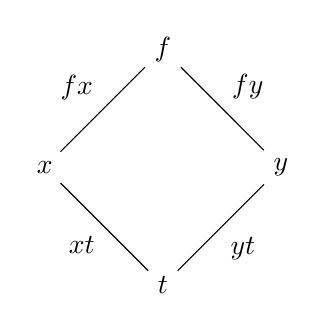
\begin{tikzpicture}
        \node (f) at (0,0) {$f$};  
        \node (x) at (-1.5,-1.5) {$x$};  
        \node (y) at (1.5,-1.5) {$y$};  
        \node (t) at (0,-3) {$t$};  
        \draw (f) edge node[midway,above left] {$\pdv{f}{x}$} (x) ;
        \draw (f) edge node[midway,above right] {$\pdv{f}{y}$} (y) ;
        \draw (x) edge node[midway,below left] {$\dv{x}{t}$} (t) ;
        \draw (y) edge node[midway,below right] {$\dv{y}{t}$} (t) ;
      \end{tikzpicture}
    \end{center}
  }{
    \begin{equation}\label{eq:deriv1}
      \dv{f}{t} = \pdv{f}{x} \dv{x}{t} + \pdv{f}{y} \dv{y}{t} 
    \end{equation}
    Ενώ η 2η παράγωγος από τον τύπο:
    \[
      \dv[2]{f}{t} =  \pdv[2]{f}{x} \left(\dv{x}{t}\right)^{2} + 
      2 \pdv[2]{f}{x}{y} \dv{x}{t} \dv{y}{t} + \pdv[2]{f}{y} 
      \left(\dv{y}{t}\right)^{2} + \pdv{f}{x} \dv[2]{x}{t} + \pdv{f}{y} \dv[2]{y}{t}
    \]
  }
\end{thm}

\section{2η Περίπτωση: \ensuremath{z=f(x,y),  x=x(u,v),  y=y(u,v)}} 

\begin{thm}
  Αν η συνάρτηση $ f(x,y) $ είναι ορισμένη στο ανοιχτό σύνολο 
  $ A \subseteq \mathbb{R}^{2} $ και $ x = x(u,v) $, $ y=y(u,v) $, με 
  και η $f$ έχει συνεχείς μερικές παραγώγους στο $A$ και οι $ x $ και $ y $, έχουν 
  συνεχείς μερικές παραγώγους στο $ E \subseteq \mathbb{R}^{2} $,
  τότε οι μερικές παράγωγοι της $f$, υπάρχουν και δίνονται από τους τύπους:
\end{thm}

\twocolumnsideslc{ 
  \begin{center}
    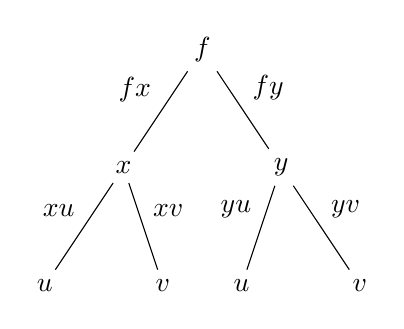
\begin{tikzpicture}
      \node (f) at (0,0) {$f$};  
      \node (x) at (-1,-1.5) {$x$};  
      \node (y) at (1,-1.5) {$y$};  
      \node (ux) at (-2,-3) {$u$};  
      \node (vx) at (-0.5,-3) {$v$};  
      \node (uy) at (0.5,-3) {$u$};  
      \node (vy) at (2,-3) {$v$};  
      \draw (f) edge node[midway,above left] {$ \pdv{f}{x}$} (x) ;
      \draw (f) edge node[midway,above right] {$ \pdv{f}{y}$} (y) ;
      \draw (x) edge node[midway,above left] {$ \pdv{x}{u}$} (ux) ;
      \draw (x) edge node[midway,above right] {$ \pdv{x}{v}$} (vx) ;
      \draw (y) edge node[midway,above left] {$ \pdv{y}{u}$} (uy) ;
      \draw (y) edge node[midway,above right] {$ \pdv{y}{v}$} (vy) ;
    \end{tikzpicture}  
  \end{center}
}{
  \begin{equation}
    \label{eq:deriv2}
    \pdv{f}{u} = \pdv{f}{x} \pdv{x}{u} + \pdv{f}{y} \pdv{y}{u} 
    \quad \text{και} \quad
    \pdv{f}{v} = \pdv{f}{x} \pdv{x}{v} + \pdv{f}{y} \pdv{y}{v} 
  \end{equation}
  Ενώ οι μερικές παράγωγοι 2ης τάξης, δίνονται από τους τύπους:
  \[
    \pdv[2]{f}{u} =  \pdv[2]{f}{x} \left(\pdv{x}{u}\right)^{2} + 
    2 \pdv[2]{f}{x}{y} \pdv{x}{u} \pdv{y}{u} + \pdv[2]{f}{y} 
    \left(\pdv{y}{u}\right)^{2} + \pdv{f}{x} \pdv[2]{x}{u} + \pdv{f}{y} 
    \pdv[2]{y}{u}
  \]
  \[
    \pdv[2]{f}{v} =  \pdv[2]{f}{x} \left(\pdv{x}{v}\right)^{2} + 
    2 \pdv[2]{f}{x}{y} \pdv{x}{u} \pdv{y}{v} + \pdv[2]{f}{y} 
    \left(\pdv{y}{v}\right)^{2} + \pdv{f}{x} \pdv[2]{x}{v} + \pdv{f}{y} 
    \pdv[2]{y}{v}
  \]
  \[
    \pdv[2]{f}{v}{u} = \pdv[2]{f}{x} \pdv{x}{u} \pdv{x}{v} + \pdv[2]{f}{x}{y}
    \left(\pdv{x}{u} \pdv{y}{v}+ \pdv{x}{v} \pdv{y}{u} \right) + \pdv[2]{f}{y} 
    \pdv{y} {u} \pdv{y}{v} + \pdv{f}{x} \pdv[2]{x}{u}{v} + \pdv{f}{y} 
    \pdv[2]{y}{u}{v} 
  \]
}


\enlargethispage{\baselineskip}

\begin{rem}
  Οι τύποι~\eqref{eq:deriv1} και~\eqref{eq:deriv2} προέκυψαν αθροίζοντας κάθε φορά, 
  τα μονοπάτια που ξεκινούν από τη μεταβλητή $f$ και καταλήγουν στη μεταβλητή ως 
  προς την οποία παραγωγίζουμε, όπου κάθε μονοπάτι αποτελείται από το γινόμενο των 
  παραγώγων που συναντούμε "διασχίζοντάς" το.
\end{rem}


\section{Αποδείξεις των τύπων των μερικών Παραγώγων 2ης τάξης}

\subsection{Απόδειξη με το συμβολισμό του Leibnitz}

Αποδεικνύουμε τον τύπο για την $ \pdv[2]{f}{u} $ και ομοίως προκύπτουν και οι τύποι 
για τις $ \pdv[2]{f}{v}  $ και $ \pdv[2]{f}{u}{v} $.

\vspace{\baselineskip}

\twocolumnsideslc
{
  \begin{center}
    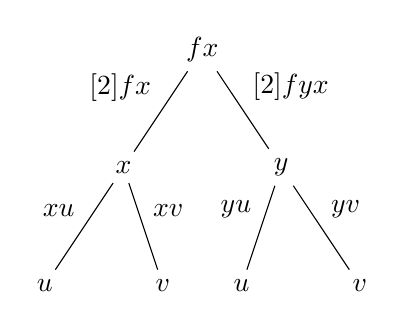
\begin{tikzpicture}
      \node (f) at (0,0) {$ \pdv{f}{x} $};  
      \node (x) at (-1,-1.5) {$x$};  
      \node (y) at (1,-1.5) {$y$};  
      \node (ux) at (-2,-3) {$u$};  
      \node (vx) at (-0.5,-3) {$v$};  
      \node (uy) at (0.5,-3) {$u$};  
      \node (vy) at (2,-3) {$v$};  
      \draw (f) edge node[midway,above left] {$ \pdv[2]{f}{x}$} (x) ;
      \draw (f) edge node[midway,above right] {$ \pdv[2]{f}{y}{x}$} (y) ;
      \draw (x) edge node[midway,above left] {$ \pdv{x}{u}$} (ux) ;
      \draw (x) edge node[midway,above right] {$ \pdv{x}{v}$} (vx) ;
      \draw (y) edge node[midway,above left] {$ \pdv{y}{u}$} (uy) ;
      \draw (y) edge node[midway,above right] {$ \pdv{y}{v}$} (vy) ;
    \end{tikzpicture}  
  \end{center}

  \begin{center}
    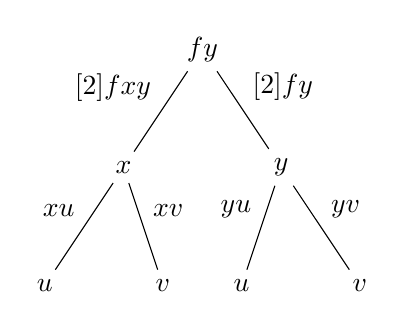
\begin{tikzpicture}
      \node (f) at (0,0) {$ \pdv{f}{y} $};  
      \node (x) at (-1,-1.5) {$x$};  
      \node (y) at (1,-1.5) {$y$};  
      \node (ux) at (-2,-3) {$u$};  
      \node (vx) at (-0.5,-3) {$v$};  
      \node (uy) at (0.5,-3) {$u$};  
      \node (vy) at (2,-3) {$v$};  
      \draw (f) edge node[midway,above left] {$ \pdv[2]{f}{x}{y}$} (x) ;
      \draw (f) edge node[midway,above right] {$ \pdv[2]{f}{y}$} (y) ;
      \draw (x) edge node[midway,above left] {$ \pdv{x}{u}$} (ux) ;
      \draw (x) edge node[midway,above right] {$ \pdv{x}{v}$} (vx) ;
      \draw (y) edge node[midway,above left] {$ \pdv{y}{u}$} (uy) ;
      \draw (y) edge node[midway,above right] {$ \pdv{y}{v}$} (vy) ;
    \end{tikzpicture}  
  \end{center}
}{
  \begin{proof}
    \[
      \begin{aligned}
        \pdv[2]{f}{u} 
  &= \pdv{}{u}\left(\pdv{f}{u}\right) = \pdv{}{u} 
  \left( \pdv{f}{x} \pdv{x}{u} + \pdv{f}{y} \pdv{y}{u}\right) = 
  \pdv{}{u} \left(\pdv{f}{x} \pdv{x}{u}\right) + \pdv{}{u} 
  \left(\pdv{f}{y} \pdv{y}{u}\right) \\
  &= \pdv{}{u} \left( \pdv{f}{x}\right) \pdv{x}{u} + \pdv{f}{x} \pdv{}{u} \left(
  \pdv{x}{u} \right) + \pdv{}{u} \left(\pdv{f}{y} \right) \pdv{y}{u} + \pdv{f}{y} 
  \pdv{}{u} \left(\pdv{y}{u}\right) \\
  &=\left[ \pdv[2]{f}{x} \pdv{x}{u} + \pdv[2]{f}{x}{y} \pdv{y}{u} \right] \pdv{x}{u} +
  \pdv{f}{x} \pdv[2]{x}{u} + 
  \left[ \pdv[2]{f}{y}{x} \pdv{x}{u} + \pdv[2]{f}{y} \pdv{y}{u} \right] \pdv{y}{u} +
  \pdv{f}{y} \pdv[2]{y}{u} \\
  &= \pdv[2]{f}{x} \left(\pdv{x}{u}\right)^{2} + \pdv[2]{f}{x}{y} \pdv{y}{u}
  \pdv{x}{u} + \pdv{f}{x} \pdv[2]{x}{u} + \pdv[2]{f}{y}{x} \pdv{x}{u} \pdv{y}{u} + 
  \pdv[2]{f}{y} \left(\pdv{y}{u}\right)^{2} +
  \pdv{f}{y} \pdv[2]{y}{u} \\
  &= \pdv[2]{f}{x} \left(\pdv{x}{u}\right)^{2} + 2\pdv[2]{f}{x}{y} \pdv{x}{u}
  \pdv{y}{u} + \pdv[2]{f}{y} \left(\pdv{y}{u}\right)^{2} + \pdv{f}{x} \pdv[2]{x}{u} +
  \pdv{f}{y} \pdv[2]{y}{u} \\
      \end{aligned}
    \]
  \end{proof}
}


\subsection{Απόδειξη με το συμβολισμό των δεικτών}

Αποδεικνύουμε τον τύπο για την $ f_{uu} $ και ομοίως προκύπτουν και οι τύποι για τις  
$ f_{vv} $ και $ f_{uv} $.

\vspace{\baselineskip}

\twocolumnsideslc{
\begin{center}
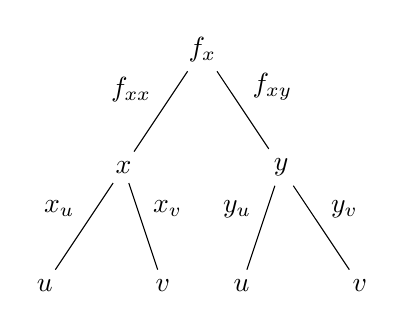
\begin{tikzpicture}
  \node (f) at (0,0) {$f_{x}$};  
  \node (x) at (-1,-1.5) {$x$};  
  \node (y) at (1,-1.5) {$y$};  
  \node (ux) at (-2,-3) {$u$};  
  \node (vx) at (-0.5,-3) {$v$};  
  \node (uy) at (0.5,-3) {$u$};  
  \node (vy) at (2,-3) {$v$};  
  \draw (f) edge node[midway,above left] {$f_{xx}$} (x) ;
  \draw (f) edge node[midway,above right] {$f_{xy}$} (y) ;
  \draw (x) edge node[midway,above left] {$x_{u}$} (ux) ;
  \draw (x) edge node[midway,above right] {$x_{v}$} (vx) ;
  \draw (y) edge node[midway,above left] {$y_{u}$} (uy) ;
  \draw (y) edge node[midway,above right] {$y_{v}$} (vy) ;
\end{tikzpicture}
\end{center}

\begin{center}
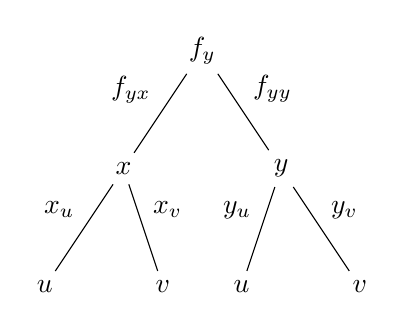
\begin{tikzpicture}
  \node (f) at (0,0) {$f_{y}$};  
  \node (x) at (-1,-1.5) {$x$};  
  \node (y) at (1,-1.5) {$y$};  
  \node (ux) at (-2,-3) {$u$};  
  \node (vx) at (-0.5,-3) {$v$};  
  \node (uy) at (0.5,-3) {$u$};  
  \node (vy) at (2,-3) {$v$};  
  \draw (f) edge node[midway,above left] {$f_{yx}$} (x) ;
  \draw (f) edge node[midway,above right] {$f_{yy}$} (y) ;
  \draw (x) edge node[midway,above left] {$x_{u}$} (ux) ;
  \draw (x) edge node[midway,above right] {$x_{v}$} (vx) ;
  \draw (y) edge node[midway,above left] {$y_{u}$} (uy) ;
  \draw (y) edge node[midway,above right] {$y_{v}$} (vy) ;
\end{tikzpicture}
\end{center}
}{
  \begin{proof}
    \[
      \begin{aligned}
        f_{uu} &= (f_{u})_{u} = (f_{x}x_{u}+f_{y}y_{u})_{u} \\
               &=(f_{x}x_{u})_{u}+ (f_{y}y_{u})_{u} \\
               &=(f_{x})_{u}x_{u} + f_{x}(x_{u})_{u} + (f_{y})_{u}y_{u}+ 
               f_{y}(y_{u})_{u} \\
               &= (f_{xx}x_{u}+f_{xy}{y_{u}})x_{u} + f_{x} x_{uu} + 
               (f_{yx}x_{u}+f_{yy}y_{u})y_{u} + f_{y}y_{uu} \\
               &= f_{xx}(x_{u})^{2} + f_{xy}y_{u}x_{u}+ f_{x}x_{uu} + 
               f_{yx}x_{u}y_{u}+f_{yy}(y_{u})^{2}+ f_{y}y_{uu} \\
               &= f_{xx}(x_{u})^{2}+ 2f_{xy}x_{u}y_{u} + f_{yy}(y_{u})^{2} + 
               f_{x}x_{uu} + f_{y}y_{uu}
      \end{aligned}
    \] 
  \end{proof}
}

\begin{rem}
  Συγκεντρωτικά οι τύποι για τις παραγώγους 2ης τάξης της συνάρτησης 
  \[
    f_{uu}= f_{xx}(x_{u})^{2}+ 2f_{xy}x_{u}y_{u} + f_{yy}(y_{u})^{2} + f_{x}x_{uu} + 
    f_{y}y_{uu} 
  \] 
  \[
    f_{vv}= f_{xx}(x_{v})^{2}+ 2f_{xy}x_{v}y_{v} + f_{yy}(y_{v})^{2} + f_{x}x_{vv} + 
    f_{y}y_{vv} 
  \]
  \[
    f_{uv}= f_{xx}x_{u}x_{v}+ f_{xy}(x_{u}y_{v} + x_{v}y_{u}) + 
    f_{yy}y_{u}y_{v} + f_{x}x_{uv} + f_{y}y_{v} 
    f_{y}y_{vv} 
  \]
\end{rem}


\chapter{Ομογενείς Συναρτήσεις}

\section{Ορισμός}

\begin{dfn}
\item {}
  \begin{enumerate}[i)]
    \item $ f(x,y) $ \textcolor{Col1}{ομογενής βαθμού} $ \textcolor{Col1}{\rho} 
      \Leftrightarrow f(\lambda x, \lambda y), \; \forall \lambda \in \mathbb{R} $ 
    \item $ f(x,y,z) $ \textcolor{Col1}{ομογενής βαθμού} $ \textcolor{Col1}{\rho} 
      \Leftrightarrow f(\lambda x, \lambda y, \lambda z), \; \forall \lambda \in 
      \mathbb{R} $ 
  \end{enumerate}
\end{dfn}

\begin{thm}[Euler]
  Αν $ f(x,y) $ είναι ομογενής βαθμού $ \rho $ τότε $x f_{x} + y f_{y} = \rho f $.
\end{thm}
\begin{prop}
  Αν $ f(x,y) $ είναι ομογενής βαθμού $ \rho $ τότε οι συναρτήσεις 
  $f_{x}, f_{y} $ είναι ομογενείς βαθμού $ \rho -1 $.
\end{prop}
\begin{proof}
\item {}
  $ f $ ομογενής βαθμού $ \rho \overset{\text{(Euler)}}{\Rightarrow} xf_{x}+yf_{y}= 
  \rho f \xRightarrow[\text{ως προς $x$}]{\text{παρ/ζω}} f_{x} + x f_{xx} + y f_{yx} =
  \rho f_{x} \Rightarrow xf_{xx} + yf_{xy} = (\rho -1)f_{x} $

  $ f $ ομογενής βαθμού $ \rho \overset{\text{(Euler)}}{\Rightarrow} xf_{x}+yf_{y}= 
  \rho f \xRightarrow[\text{ως προς $y$}]{\text{παρ/ζω}} xf_{xy} + f_{y} + y f_{yy} =
  \rho f_{y} \Rightarrow xf_{yx} + yf_{yy} = (\rho -1)f_{y} $
\end{proof}

\begin{exercise}
  Έστω $ f(x,y) $, συνεχής, με συνεχείς μερικές παραγώγους 2ης τάξης, 
  ομογενής βαθμού $\rho$. Να δείξετε ότι ισχύει \[ x^{2}f_{xx}+2xyf_{xy}+y^{2}f_{yy} =
  \rho (\rho -1)f \]
\end{exercise}
\begin{solution}
\item {}
  $f$ ομογενής βαθμού $\rho \Rightarrow f_{x}, f_{y} $ ομογενείς βαθμού $\rho -1$.
  Οπότε ισχύει το θεώρημα Euler για αυτές, άρα:
  \begin{align*}
    \sysdelim.\}\systeme{x f_{xx}+yf_{xy}=(\rho -1)f_{x}, x f_{yx}+yf_{yy}=
  (\rho -1)f_{y}} \Rightarrow \sysdelim.\}
  \systeme*{x^{2} f_{xx} \+ xyf_{xy}=(\rho-1)xf_{x},yxf_{yx} \+ y^{2}f_{yy}=
  (\rho -1)yf_{y}} \xRightarrow{(+)} x^{2}f_{xx}+2xyf_{xy}+y^{2}f_{yy}=
  (\rho -1)(xf_{x}+yf_{y})
\end{align*} 
Όμως επειδή $f$ ομογενής έχουμε ότι $ xf_{x}+yf_{y}= \rho f $. Οπότε
\[
  x^{2}f_{xx}+2xyf_{xy}+y^{2}f_{yy} = \rho (\rho -1)f
\] 
\end{solution}


\begin{exercise}
  Αν $ u = u(x,y) $ και $ v=v(x,y) $ ομογενείς βαθμού $ \rho $, 
  τότε να δείξετε ότι $ \forall f(u,v) $ με συνεχείς μερικές παραγώγους 1ης τάξης
  ισχύει 
  \[
    xf_{x}+yf_{y}= \rho (u f_{u}+vf_{v}) 
  \] 
\end{exercise}
\begin{solution}
\item {}
  Έχουμε ότι για τις συναρτήσεις $u(x,y) $ και $v(x,y)$ είναι ομογενείς 
  βαθμού $\rho$, οπότε:
  \[
  \sysdelim.\}\systeme{xu_{x}+yu_{y}= \rho u, xv_{x}+yv_{y}= \rho v} 
\] 
Για την συνάρτηση $f$ έχουμε ότι είναι σύνθετη με $ f=f(u,v) $ και 
$ u = u(x,y) $ και $ v=v(x,y) $, οπότε οι μερικές παράγωγοί της δίνονται από
το δέντρο της και είναι:
\[
  \left.
    \begin{tabular}{l}
      $f_{x}=f_{u}u_{x}+f_{v}v_{x}$ \\
      $f_{y}=f_{u}u_{y}+f_{v}v_{y}$
    \end{tabular}
  \right\}
  \Rightarrow xf_{x}+yf_{y} = \underbrace{(xu_{x}+yu_{y})}_{\rho
  u}f_{u}+\underbrace{(xv_{x}+yv_{y})}_{\rho v}f_{v}
\] 
Άρα 
\[
  xf_{x}+yf_{y} = \rho (uf_{u}+vf_{v}) 
\] 
\end{solution}

\begin{exercise}
  Έστω $ u = u(x,y) $ και $ v = v(x,y) $, ομογενείς βαθμού $\rho$, με 
  $ u(x,y) \neq 0, v(x,y) \neq 0, \; \forall (x,y) \in \mathbb{R}^{2} $. 
  Να δείξετε ότι 
  \[
    udv -v du = \frac{1}{\rho} \pdv{(u,v)}{(x,y)} (xdy-ydx) 
    \quad \text{όπου} \quad  \pdv{(u,v)}{(x,y)} = 
    \begin{vmatrix}
      u_{x} & u_{y} \\ v_{x} & v_{y} 
    \end{vmatrix} 
  \] 
\end{exercise}
\begin{solution}
  \[
    \left.
      \begin{matrix}
        du=u_{x}dx+u_{y}dy \\
        dv=v_{x}dx+v_{y}dy
      \end{matrix} 
    \right\} \Rightarrow 
    \left.
      \begin{matrix}
        vdu=vu_{x}dx+vu_{y}dy \\ 
        udv=uv_{x}dx+uv_{y}dy
      \end{matrix} 
    \right\} \overset{(-)}{\Rightarrow} 
    udv -vdu = (uv_{x}-vu_{x})dx+(uv_{y}-vu_{y})dy 
  \] 

  \begin{align*}
    u \quad \text{ομογενής βαθμού $\rho$} \Rightarrow xu_{x}+yu_{y}= 
    \rho u \Rightarrow u &= \frac{1}{\rho} (xu_{x}+yu_{y})   \\
    v \quad \text{ομογενής βαθμού $\rho$} \Rightarrow xv_{x}+yv_{y}= 
    \rho v \Rightarrow u &= \frac{1}{\rho} (xv_{x}+yv_{y})   
  \end{align*} 
  Οπότε με αντικατάσταση, έχουμε:
  \begin{align*}
    udv - vdu &= \frac{1}{\rho} (u_{y}v_{x}-u_{x}v_{y})ydx+ \frac{1}{\rho}
    (u_{x}v_{y}-u_{y}v_{x})xdy \\ 
              &=- \frac{1}{\rho} (u_{x}v_{y}-u_{y}v_{x})ydx+ \frac{1}{\rho}
              (u_{x}v_{y}-u_{y}v_{x})xdy \\
              &= \frac{1}{\rho} (u_{x}v_{y}-u_{y}v_{x})(xdy-ydx) \\
              &= \frac{1}{\rho} \cdot \pdv{(u,v)}{(x,y)} (xdy-ydx)
  \end{align*}
\end{solution}



\chapter{Πεπλεγμένες Συναρτήσεις}


\section{Θεωρήματα Πεπλεγμένων συναρτήσεων}

\vspace{\baselineskip}

\subsection{Η εξίσωση \ensuremath{F(x,y) = 0}}

\subsubsection{Πεπλεγμένη συνάρτηση της μορφής \ensuremath{y=f(x)}}

Έστω $ F(x,y) = 0 $, όπου $ F\colon D \to \mathbb{R} $ μια συνάρτηση με πεδίο
ορισμού ένα ανοιχτό υποσύνολο $D$ του $\mathbb{R}^{2}$ και $ (x_0,y_0) $ ένα 
εσωτερικό σημείο του $D$.  Αν 
\begin{enumerate}[(i)]
  \item $F(x_0,y_0) = 0$ 
  \item $ F_x, F_y$ συνεχείς σε περιοχή του σημείου $ (x_0,y_0) $ 
  \item $ F_{\textcolor{Col1}{y}}(x_0,y_0) \neq 0 $
\end{enumerate}
τότε υπάρχει μοναδική συνάρτηση $\textcolor{Col1}{y=y(x)} $ ορισμένη στο 
$ I_0 \subseteq \mathbb{R} $ τέτοια ώστε:
\begin{myitemize}
  \item $y_0 = y(x_0)$
  \item $F(x,y(x)) = 0, \quad \forall x \in I_0$
  \item $ \dv{y}{x} = - \frac{F_x}{F_y}, \quad \forall x \in I_0  $
\end{myitemize}

\begin{rem}
  Ο παραπάνω τύπος για την παράγωγο $ \dv{y}{x} $ προκύπτει ως λύση της εξίσωσης
  \[
    \pdv{F}{x} + \pdv{F}{y}\dv{y}{x} = 0 
  \] 
  η οποία προκύπτει με παραγώγιση της $ F(x,y) = 0$, αν θεωρήσουμε ότι $ y=y(x) $.
\end{rem}

\subsubsection{Πεπλεγμένη συνάρτηση της μορφής \ensuremath{x=f(y)}}

Έστω $ F(x,y) = 0 $, όπου $ F\colon D \to \mathbb{R} $ μια συνάρτηση με πεδίο
ορισμού ένα ανοιχτό υποσύνολο $D$ του $\mathbb{R}^{2}$ και $ (x_0,y_0) $ ένα 
εσωτερικό σημείο του $D$.  Αν 
\begin{enumerate}[(i)]
  \item $F(x_0,y_0) = 0$ 
  \item $ F_x, F_y$ συνεχείς σε περιοχή του σημείου $ (x_0,y_0) $ 
  \item $ F_{\textcolor{Col1}{x}}(x_0,y_0) \neq 0 $
\end{enumerate}
τότε υπάρχει μοναδική συνάρτηση $ \textcolor{Col1}{x=x(y)} $ ορισμένη στο 
$ I_0 \subseteq \mathbb{R} $ τέτοια ώστε:
\begin{myitemize}
  \item $x_0 = x(y_0)$
  \item $F(x(y),y) = 0, \quad \forall y \in I_0$
  \item $ \dv{x}{y} = - \frac{F_y}{F_x}, \quad \forall y \in I_0  $
\end{myitemize}

\begin{rem}
  Ο παραπάνω τύπος για την παράγωγο $ \dv{x}{y} $ προκύπτει ως λύση της εξίσωσης
  \[
    \pdv{F}{y} + \pdv{F}{x}\dv{x}{y} = 0 
  \] 
  η οποία προκύπτει με παραγώγιση της $ F(x,y) = 0$, αν θεωρήσουμε ότι $ x=x(y) $.
\end{rem}
\begin{example}
  Να υπολογίσετε τα σημεία της καμπύλης $ F(x,y) = x^{3}+y^{3}-6xy=0 $ για τα οποία 
  ισχύει το θεώρημα πεπλεγμένης συνάρτησης.
\end{example}
\begin{solution}
  Αρχικά εξετάζουμε αν το $ y $ μπορεί να είναι πεπλεγμένη συνάρτηση του $x$.   
  Βρίσκουμε τα σημεία που επαληθεύουν την εξίσωση και για τα οποία $ F_{y}=0 $.
  \[
    F_{y} = 0 \Leftrightarrow 3y^{2}-6x=0 \Leftrightarrow \inlineequation[xsom]
    {x = \frac{1}{2} y^{2}}
  \] 
  Βρίσκουμε ποια από αυτά τα σημεία επαληθεύουν την εξίσωση και έχουμε:
  \[
    \left(\frac{1}{2} y^{2}\right)^{3}+y^{3}-6 \frac{1}{2} y^{2}y=0 
    \Leftrightarrow \frac{1}{8} y^{6}+y^{3} -3y^{3}=0 
    \Leftrightarrow y^{3}\left(\frac{1}{8} y^{3}-2\right)=0 \Leftrightarrow y=0 \quad
    \text{ή} \quad y= \sqrt[3]{16} = \sqrt[3]{8\cdot2} = 2 \sqrt[3]{2}
  \] 
  Άρα, από την εξίσωση~\eqref{xsom} έχουμε ότι 
  \[ 
    x=0  \quad \text{ή} \quad x = \frac{1}{2} \left(2 \sqrt[3]{2}\right)^{2} = 
    \frac{1}{2} \left(2 \cdot 2^{\frac{1}{3}}\right)^{2} = 2 \cdot 2^{\frac{2}{3}} 
    = 2 \sqrt[3]{2^{2}} = 2 \sqrt[3]{4}  
  \]
  Επομέvως το θεώρημα δεν εφαρμόζεται για τα σημεία $ (0,0) $ και $ (2 \sqrt[3]{4}
  , 2 \sqrt[3]{2}) $.

  Στη συνέχεια εξετάζουμε αν το $ x $ μπορεί να είναι πεπλεγμένη συνάρτηση του $y$.
  Βρίσκουμε τα σημεία που επαληθεύουν την εξίσωση και για τα οποία $ F_{x}=0 $.
  \[
    F_{x}=0 \Leftrightarrow 3x^{2}-6y=0 \Leftrightarrow \inlineequation[ysom]
    {y= \frac{1}{2} x^{2}}
  \] 
  Βρίσκουμε ποια από αυτά τα σημεία επαληθεύουν την εξίσωση και έχουμε:
  \[
    x^{3}+\left(\frac{1}{2} x^{2}\right)^{3}-6x \frac{1}{2} x^{2}=0 \Leftrightarrow 
    x^{3}+ \frac{1}{8} x^{6}-3x^{3}=0 \Leftrightarrow \frac{1}{8} x^{6}-3x^{3}=0
    \Leftrightarrow x^{3}\left(\frac{1}{8} x^{3}-2\right)=0 \Leftrightarrow x = 0 \quad
    \text{ή} \quad x=2 \sqrt[3]{2} 
  \] 
  Άρα, από την εξίσωση~\eqref{ysom} έχουμε ότι 
  \[ 
    y=0  \quad \text{ή} \quad y = 2 \sqrt[3]{4} 
  \]
  Επομέvως το θεώρημα δεν εφαρμόζεται για τα σημεία $ (0,0) $ και $ (2 \sqrt[3]{2}
  , 2 \sqrt[3]{4}) $.

  Οπότε συνολικά, το θεώρημα δεν εφαρμόζεται για τα σημεία 
  \[
    \boxed{(0,0), \quad (2 \sqrt[3]{4} , 2 \sqrt[3]{2}), \quad (2 \sqrt[3]{2} , 2
    \sqrt[3]{4})}
  \] 
\end{solution}

\subsection{Η εξίσωση \ensuremath{F(x,y,z) = 0}}

\subsubsection{Πεπλεγμένη συνάρτηση της μορφής \ensuremath{z=z(x,y)}}

Έστω $ F(x,y,z) = 0 $, όπου $F\colon D \to \mathbb{R}$ μια συνάρτηση με πεδίο ορισμού 
ένα ανοικτό υποσύνολο $ D $ του $ \mathbb{R}^{3}  $ και $ (x_0,y_0,z_0) $ ένα 
εσωτερικό σημείο του $ D $. Αν
\begin{enumerate}[(i)]
  \item $ F(x_0,y_0,z_0) $
  \item $ F_x, F_y, F_z $ συνεχείς σε περιοχή του σημείου $ (x_0,y_0,z_0) $
  \item $ F_{\textcolor{Col1}{z}}(x_0,y_0,z_0) \neq 0 $
\end{enumerate}
τότε υπάρχει μοναδική συνάρτηση, $ \textcolor{Col1}{z=z(x,y)} $ ορισμένη στο 
$ D_0 \subseteq \mathbb{R}^{2} $ τέτοια ώστε:
\begin{myitemize}
  \item $ z_0 = z(x_0,y_0) $
  \item $ F(x,y,z(x,y)) = 0,  \quad \forall (x,y)\in  D_0 $
  \item $ \pdv{z}{x} = - \frac{F_x}{F_z} $ και $ \pdv{z}{y} = - \frac{F_y}{F_z}, 
    \quad \forall (x,y) \in D_0$
\end{myitemize}

\begin{rem}
  Οι παραπάνω τύποι για τις παραγώγους $ \pdv{z}{x}, \pdv{z}{y} $ προκύπτουν 
  ως λύσεις των εξισώσεων  
  \begin{align*}	
    \pdv{F}{x} + \pdv{F}{z}\pdv{z}{x} &= 0 \\
    \pdv{F}{y} + \pdv{F}{z}\pdv{z}{y} &= 0 
  \end{align*}
  οι οποίες προκύπτουν με παραγώγιση της $ F(x,y,z) = 0 $, ως προς $x$ και $y$ 
  αντίστοιχα και  αν θεωρήσουμε ότι $ z=z(x,y) $.
\end{rem}

\subsubsection{Πεπλεγμένη συνάρτηση της μορφής \ensuremath{y=y(x,z)}}

Έστω $ F(x,y,z) = 0 $, όπου $F\colon D \to \mathbb{R}$ μια συνάρτηση με πεδίο ορισμού 
ένα ανοικτό υποσύνολο $ D $ του $ \mathbb{R}^{3}  $ και $ (x_0,y_0,z_0) $ ένα 
εσωτερικό σημείο του $ D $. Αν
\begin{enumerate}[(i)]
  \item $ F(x_0,y_0,z_0) $
  \item $ F_x, F_y, F_z $ συνεχείς σε περιοχή του σημείου $ (x_0,y_0,z_0) $
  \item $ F_{\textcolor{Col1}{y}}(x_0,y_0,z_0) \neq 0 $
\end{enumerate}
τότε υπάρχει μοναδική συνάρτηση, $ \textcolor{Col1}{y=y(x,z)} $ ορισμένη στο 
$ D_0 \subseteq \mathbb{R}^{2} $ τέτοια ώστε:
\begin{myitemize}
  \item $ y_0 = y(x_0,z_0) $
  \item $ F(x,y(x,z),z)) = 0,  \quad \forall (x,z) \in  D_0 $
  \item $ \pdv{y}{x} = - \frac{F_x}{F_y} $ και $ \pdv{y}{z} = - \frac{F_z}{F_y}, 
    \quad \forall (x,z) \in D_0$
\end{myitemize}

\begin{rem}
  Οι παραπάνω τύποι για τις παραγώγους $ \pdv{y}{x}, \pdv{y}{z} $ προκύπτουν 
  ως λύσεις των εξισώσεων  
  \begin{align*}	
    \pdv{F}{x} + \pdv{F}{y}\pdv{y}{x} &= 0 \\
    \pdv{F}{z} + \pdv{F}{y}\pdv{y}{z} &= 0 
  \end{align*}
  οι οποίες προκύπτουν με παραγώγιση της $ F(x,y,z) = 0 $, ως προς $x$ και $z$ 
  αντίστοιχα και  αν θεωρήσουμε ότι $ y=y(x,z) $.
\end{rem}

\subsubsection{Πεπλεγμένη συνάρτηση της μορφής \ensuremath{x=x(y,z)}}

Έστω $ F(x,y,z) = 0 $, όπου $F\colon D \to \mathbb{R}$ μια συνάρτηση με πεδίο ορισμού 
ένα ανοικτό υποσύνολο $ D $ του $ \mathbb{R}^{3}  $ και $ (x_0,y_0,z_0) $ ένα 
εσωτερικό σημείο του $ D $. Αν
\begin{enumerate}[(i)]
  \item $ F(x_0,y_0,z_0) $
  \item $ F_x, F_y, F_z $ συνεχείς σε περιοχή του σημείου $ (x_0,y_0,z_0) $
  \item $ F_{\textcolor{Col1}{x}}(x_0,y_0,z_0) \neq 0 $
\end{enumerate}
τότε υπάρχει μοναδική συνάρτηση, $ \textcolor{Col1}{x=x(y,z)} $ ορισμένη στο 
$ D_0 \subseteq \mathbb{R}^{2} $ τέτοια ώστε:
\begin{myitemize}
  \item $ x_0 = x(y_0,z_0) $
  \item $ F(x(y,z),y,z)) = 0,  \quad \forall (y,z) \in  D_0 $
  \item $ \pdv{x}{y} = - \frac{F_y}{F_x} $ και $ \pdv{x}{z} = - \frac{F_z}{F_x}, 
    \quad \forall (y,z) \in D_0$
\end{myitemize}

\begin{rem}
  Οι παραπάνω τύποι για τις παραγώγους $ \pdv{x}{y}, \pdv{x}{z} $ προκύπτουν 
  ως λύσεις των εξισώσεων  
  \begin{align*}	
    \pdv{F}{y} + \pdv{F}{x}\pdv{x}{y} &= 0 \\
    \pdv{F}{z} + \pdv{F}{x}\pdv{x}{z} &= 0 
  \end{align*}
  οι οποίες προκύπτουν με παραγώγιση της $ F(x,y,z) = 0 $, ως προς $y$ και $z$ 
  αντίστοιχα και  αν θεωρήσουμε ότι $ x=x(x,z) $.
\end{rem}
\begin{example}
  Έστω η εξίσωση $ F(x,y,z) = y^{2}+xz+z^{2}- \mathrm{e}^{z}-4 = 0$. 
  Να εξετάσετε αν ισχύει το θεώρημα πεπλεγμένης συνάρτησης, για την 
  $ z = z(x,y) $, στο σημείο $P(0,\mathrm{e},2) $ και να βρεθούν οι μερικές παράγωγοι 
  1ης και 2ης τάξης της συνάρτησης $ z = z(x,y) $ στο σημείο $ (0, \mathrm{e}) $.
\end{example}
\begin{solution}
\item {}
  \begin{enumerate}[i)]
    \item $ F(0, \mathrm{e}, 2) = \mathrm{e}^{2} + 0\cdot 2 + 2^{2} - 
      \mathrm{e}^{2} - 4 = 0  $ 
    \item 
      \begin{tabular}{l}
        $ F_{x} = z \phantom{\ +2z- \mathrm{e}^{z}} $ \tikzmark{a} \\
        $ F_{y} = 2y $ \\
        $ F_{z} = x+2z- \mathrm{e}^{z} \tikzmark{b} $
      \end{tabular}
      \mybrace{a}{b}[είναι συνεχείς ως πολυωνυμικές]
    \item $ F_{z}(0, \mathrm{e},2) = 0+2\cdot 2- \mathrm{e}^{2} 
      = 4- \mathrm{e}^{2} \neq 0 $
  \end{enumerate}
  Επομένως ικανοποιούνται οι προϋποθέσεις του θεωρήματος Πεπλεγμένης συνάρτησης 
  και άρα υπάρχει μοναδική συνάρτηση $ z=z(x,y) $, για την οποία ισχύουν:
  \begin{myitemize}
    \item $ \inlineequation[eq:perplex1]{2=z(0, \mathrm{e})} $
    \item $ z_{x} = - \frac{F_{x}}{F_{z}} = - \frac{z}{x+2z- \mathrm{e}^{z}} $ και 
      $ z_{y} = - \frac{F_{y}}{F_{z}} - \frac{2y}{x+2z- \mathrm{e}^{z}} $ σε μια 
      περιοχή του σημείου $ (0,\mathrm{e}) $.
  \end{myitemize}
  Επομένως στο σημείο $ (0, \mathrm{e}) $ έχουμε ότι $ z= z(0, \mathrm{e}) = 2 $ και 
  άρα:
  \[
    z_{x}(0, \mathrm{e}) \overset{\eqref{eq:perplex1}}{=}  
    - \frac{2}{0+2\cdot 2- e^{2}} = - \frac{2}{4-\mathrm{e}^{2}} \quad \text{και} 
    \quad z_{y}(0, \mathrm{e}) \overset{\eqref{eq:perplex1}}{=}  
    - \frac{2 \cdot \mathrm{e}}{0+2\cdot 2 - 
    \mathrm{e}^{2}} = - \frac{2 \mathrm{e}}{4- \mathrm{e}^{2}} 
  \]
  Για να βρούμε τις μερικές παραγώγους 2ης τάξης της συνάρτησης $ z(x,y) $, 
  παραγωγίζουμε ξανά, τις μερικές παραγώγους 1ης τάξης, θεωρούμε όμως ότι 
  $z=z(x,y)$ είναι συνάρτηση.
  \begin{align*}
    z_{xx} &= \left(\frac{-z}{x+2z- \mathrm{e}^{z}}\right) _{x} =
    \frac{(-z)_{x}(x+2z- \mathrm{e}^{z})-(-z)(x+2z- \mathrm{e}^{z} )_{x}}{(x+2z-
      \mathrm{e}^{z})^{2}} = \frac{-z_{x}(x+2z- \mathrm{e}^{z})+z(1+2z_{x}- 
    \mathrm{e}^{z} z_{x})}{(x+2z- \mathrm{e}^{z})^{2}}  \\ 
    z_{yy} &= \left(\frac{-2y}{x+2z- \mathrm{e}^{z}}\right)_{y} = 
    \frac{(-2y)_{y}(x+2z- \mathrm{e}^{z})- (-2y)(x+2z- \mathrm{e}^{z} )_{y}}{(x+2z-
      \mathrm{e}^{z} )^{2}} = \frac{(-2)(x+2z- \mathrm{e}^{z} )+2y(2z_{y}-
    \mathrm{e}^{z} z_{y})}{(x+2z- \mathrm{e}^{z})^{2}} \\  
    z_{xy}&= \left(\frac{-z}{x+2z+ \mathrm{e}^{z}}\right)_{y} = 
    \frac{(-z)_{y}(x+2z+ \mathrm{e}^{z})-(-z)(x+2z+ \mathrm{e}^{z} )_{y}}{(x+2z+
      \mathrm{e}^{z})^{2}} = \frac{-z_{y}(x+2z+ \mathrm{e}^{z})+z(+2z_{y}+ 
    \mathrm{e}^{z} z_{y})}{(x+2z+ \mathrm{e}^{z})^{2}}  \\ 
  \end{align*} 
\end{solution}

Με αντικατάσταση, όπου $ (x,y,z)=(0, \mathrm{e}, 2) $ αλλά και όπου $ z_{x}$ και 
$ z_{y} $ τις τιμές που μόλις βρήκαμε, υπολογίζουμε και τις τιμές των παραγώγων 2ης
τάξης στο σημείο $ (0, \mathrm{e}) $.

% \enlargethispage{\baselineskip}

% Επομένως στο σημείο $ (0, \mathrm{e}) $ έχουμε ότι $ z= z(0, \mathrm{e}) = 2 $, 
% $ z_{x}(0, \mathrm{e}) = - \frac{2}{4- \mathrm{e}^{2}} $ και $ z_{y}(0, \mathrm{e}) 
% = - \frac{2 \mathrm{e}}{4 - \mathrm{e}^{2}}$ και άρα:
% \begin{align*}
%   z_{xx}(0, \mathrm{e}) &= \frac{ \frac{2}{4-\mathrm{e}^{2}}(0+2\cdot 2-
%     \mathrm{e}^{2})+2[1+2 (-\frac{2}{4-\mathrm{e}^{2}}) - \mathrm{e}^{2}
%   (-\frac{2}{4-\mathrm{e}^{2}})]}{(0+2 \cdot 2 - \mathrm{e}^{2})^{2}} = 
%   \frac{2 + \frac{2 \mathrm{e}^{2}}{4- \mathrm{e}^{2}}}{(4- \mathrm{e}^{2})^{2}} 
%   = \frac{8}{(4- \mathrm{e}^{2})^{3}} \\
%     z_{yy}(0, \mathrm{e}) &= \frac{(-2)(0+2 \cdot 2 - \mathrm{e}^{2})+2 
%       \mathrm{e}[2\cdot (-\frac{2 \mathrm{e}}{4- \mathrm{e}^{2}}) - 
%       \mathrm{e}^{2} (-\frac{2 \mathrm{e}}{4- \mathrm{e}^{2}})]}{(4- 
%       \mathrm{e}^{2})^{2}} = \frac{-8+2 \mathrm{e}^{2}-
%       \frac{8e^{2}}{4- \mathrm{e}^{2}}+ \frac{4e^{3}}{4- \mathrm{e}^{2}}}{(4-
%       \mathrm{e}^{2})^{2}} = \frac{2(\mathrm{e}^{4} + 4 \mathrm{e}^{2} -16)}{(4-
%     \mathrm{e}^{2})^{2}} 
%     \end{align*}


\subsection{Συστήματα Εξισώσεων}

\subsubsection{1η περίπτωση}

Έστω το σύστημα εξισώσεων $(\Sigma):
\begin{cases}
  F(x,y,z) = 0  \\
  G(x,y,z) = 0
\end{cases}$
και έστω το σημείο $ P_0(x_0,y_0,z_0) $, όπου ισχύει:
\begin{enumerate}[(i)]
  \item  
    \begin{tabular}{l}
      $F(x_0,y_0,z_0) = 0$ \\
      $G(x_0,y_0,z_0) = 0$
    \end{tabular}
  \item Οι συναρτήσεις $ F, G $ είναι $ C^{1} $ τάξης 
  \item $ \eval{\pdv{(F,G)}{(y,z)}} _{P_{0}} \neq 0 $
\end{enumerate} 
τότε υπάρχουν μοναδικές συναρτήσεις $ y = y(x) $ και $ z = z(x) $ τάξης $ C^{1} $ 
τέτοιες ώστε:
\begin{myitemize}
  \item 
    \begin{tabular}{l}
      $ y_0 = y(x_0) $ \\
      $ z_0 = z(x_0) $
    \end{tabular}
  \item 
    \begin{tabular}{l}
      $ F(x,y(x),z(x)) = 0 $ \\
      $ G(x,y(x),z(x)) = 0 $
    \end{tabular}
  \item $ \dv{y}{x} = - \frac{\pdv{(F,G)}{(x,z)}}{\pdv{(F,G)}{(y,z)}} $ και 
    $ \dv{z}{x} = - \frac{\pdv{(F,G)}{(y,x)}}{\pdv{(F,G)}{(y,z)}} $
\end{myitemize}

\begin{rem}
  Οι παραπάνω τύποι για τις τιμές των μερικών παραγώγων $ \dv{y}{x}, \dv{z}{x}$ 
  προκύπτουν ως λύσεις του ακόλουθου $ 2 \times 2 $ συστήματος εξισώσεων οι οποίες 
  προκύπτουν με παραγώγιση των εξισώσεων του συστήματος $ (\Sigma) $, ως προς $x$.
  \renewcommand{\arraystretch}{2}
  \[
    \begin{aligned}
      (\Sigma_x): \left\{\begin{tabular}{l}
          $\pdv{F}{x} + \pdv{F}{y}\dv{y}{x} + \pdv{F}{z}\dv{z}{x} = 0$ \\
          $\pdv{G}{x} + \pdv{G}{y}\dv{y}{x} + \pdv{G}{z}\dv{z}{x} = 0$
        \end{tabular}
      \right.
    \end{aligned}
  \]
\end{rem}

\subsubsection{2η περίπτωση}

Έστω το σύστημα εξισώσεων $(\Sigma):
\begin{cases}
  F(x,y,z,w) = 0  \\
  G(x,y,z,w) = 0
\end{cases}$
και έστω το σημείο $ P_0(x_0,y_0,z_0,w_0) $, όπου ισχύει:
\begin{enumerate}[(i)]
  \item  \begin{tabular}{l}
      $F(x_0,y_0,z_0,w_0) = 0$ \\
      $G(x_0,y_0,z_0,w_0) = 0$
    \end{tabular}
  \item Οι συναρτήσεις $ F, G $ είναι $ C^{1} $ τάξης 
  \item $ \eval{\pdv{(F,G)}{(z,w)}}_{P_0} \neq 0 $ 
\end{enumerate}
τότε υπάρχουν μοναδικές συναρτήσεις $ z = z(x,y) $ και $ w = w(x,y) $ τάξης 
$ C^{1} $ τέτοιες ώστε:
\begin{myitemize}
  \item \begin{tabular}{l}
      $ z_0 = z(x_0,y_0) $ \\
      $ w_0 = w(x_0,y_0) $
    \end{tabular}
  \item \begin{tabular}{l}
      $ F(x,y,z(x,y), w(x,y) = 0 $ \\
      $ G(x,y,z(x,y), w(x,y)) = 0 $
    \end{tabular}
  \item $ \pdv{z}{x} = - \frac{\pdv{(F,G)}{(x,w)}}{\pdv{(F,G)}{(x,w)}} $, 
    \; $ \pdv{z}{y} = - \frac{\pdv{(F,G)}{(y,w)}}{\pdv{(F,G)}{(z,w)}} $, 
    \; $ \pdv{w}{x} = - \frac{\pdv{(F,G)}{(z,x)}}{\pdv{(F,G)}{(z,w)}} $ και 
    $ \pdv{w}{y} = - \frac{\pdv{(F,G)}{(z,y)}}{\pdv{(F,G)}{(z,w)}} $
\end{myitemize}

\begin{rem}
  Οι παραπάνω τύποι για τις τιμές των μερικών παραγώγων 
  $ \pdv{z}{x}, \pdv{z}{y}, \pdv{w}{x}, \pdv{w}{y} $ προκύπτουν ως λύσεις των 
  παρακάτω $ 2 \times 2 $ γραμμικών συστημάτων τα οποία προκύπτουν με παραγώγιση 
  των εξισώσεων του συστήματος $ (\Sigma) $, ως προς $x$ και $y$ αντίστοιχα.
  \renewcommand{\arraystretch}{2}
  \[
    \begin{aligned}
      (\Sigma_x): 
      \left\{\begin{tabular}{l}
          $\pdv{F}{x} + \pdv{F}{z}\pdv{z}{x} + \pdv{F}{w}\pdv{w}{x} = 0$ \\
          $\pdv{G}{x} + \pdv{G}{z}\pdv{z}{x} + \pdv{G}{w}\pdv{w}{x} = 0$
        \end{tabular}
      \right.  &\quad \text{και} \quad& (\Sigma_y): 
      \left\{\begin{tabular}{l}
          $\pdv{F}{y} + \pdv{F}{z}\pdv{z}{y} + \pdv{F}{w}\pdv{w}{y} = 0$ \\
          $\pdv{G}{y} + \pdv{G}{z}\pdv{z}{y} + \pdv{G}{w}\pdv{w}{y} = 0$
        \end{tabular}
      \right.
    \end{aligned}
  \]
\end{rem}




\section{Ιακωβιανές Ορίζουσες}

\subsection{Ορισμός}

Έστω $ \begin{cases} 
  f^{1}=f^{1}(x_{1},\ldots,x_{n}) \\
  f^{2}=f^{2}(x_{1},\ldots,x_{n}) \\
  \vdots \\
  f^{n} = f^{n}(x_{1}\ldots,x_{n}) 
\end{cases} 
$, τότε η Ιακωβιανή ορίζουσα, είναι 
$ J = \pdv{(f^{1},\ldots,f^{n})}{(x_{1}\ldots,x_{n})} = \begin{vmatrix}
  f^{1}_{x_{1}} & f^{1}_{x_{2}} & \cdots & f^{1}_{x_{n}} \\
  f^{2}_{x_{1}} & f^{2}_{x_{2}} & \cdots & f^{2}_{x_{n}} \\
  \vdots & \vdots & \cdots & \vdots \\
  f^{n}_{x_{1}} & f^{n}_{x_{2}} & \cdots & f^{n}_{x_{n}} \\
\end{vmatrix}$

\begin{rem}
  Η κύρια χρησιμότητά τους είναι στην εύρεση των μερικών 
  παραγώγων πεπλεγμένων συναρτήσεων, όπως εξηγείται στον 
  παρακάτω γενικό κανόνα.
\end{rem}


\subsection{Γενικός Μνημονικός Κανόνας}

Όταν ζητάμε την μερική Παράγωγο μιας εξαρτημένης μεταβλητής 
$ (\text{Ε.Μ.$^{*}$}) $, ως προς κάποια ανεξάρτητη 
μεταβλητή $ (\text{Α.Μ.$^{*}$}) $, τότε αυτή είναι 
ίση με μείον το πηλίκο της Ιακωβιανής ορίζουσας 
των Πεπλεγμένων συναρτήσεων 
ως προς τις εξαρτημένες μεταβλητές όπου όμως έχουμε αντικαταστήσει την 
εξαρτημένη μεταβλητή $ (\text{Ε.Μ.$^{*}$}) $ με την ανεξάρτητη μεταβλητή 
$ (\text{Α.Μ.$^{*}$}) $ προς την Ιακωβιανή ορίζουσα των 
Πεπλεγμένων συναρτήσεων ως προς τις εξαρτημένες μεταβλητές.

\[
  \pdv{(\text{Ε.Μ.}^{*})}{(\text{Α.Μ.}^{*})} = - 
  \frac{J \; (\text{Πεπλ.\ ως προς E.M.}^{*} 
  \to A.M.^{*})}{J \; (\text{Πεπλεγμένων ως προς E.M.)}} 
\] 

\begin{example}
\item {}
  \begin{enumerate}
    \item Έστω το σύστημα
      $ \begin{cases}
        F(u,v,w,x,y)  = 0 \\
        G(u,v,w,x,y)  = 0 \\
        H(u,v,w,x,y)  = 0
      \end{cases} $. Τότε έχουμε Ε.Μ.:3 (όσες και οι 
      εξισώσεις) και Α.Μ.:2 (οι υπόλοιπες). 
      \begin{myitemize}
        \item Οπότε, αν θεωρήσουμε ως ανεξάρτητες μεταβλητές τις $x$ και $y$, τότε, 
          έχουμε:
          \[
            \left.\pdv{u}{\textcolor{Col1}{x}}\right)_{y} = - 
            \frac{\pdv{(F,G,H)}{(\textcolor{Col1}{x},v,w)}}{\pdv{(F,G,H)}{(u,v,w)}}  
            \quad \text{και} \quad \left. \pdv{v}{\textcolor{Col1}{y}} \right)_{x} = - 
            \frac{\pdv{(F,G,H)}{(u,\textcolor{Col1}{y},w)}}{\pdv{(F,G,H)}{(u,v,w)}} 
            \quad \text{και} \quad
            \left.\pdv{w}{\textcolor{Col1}{y}}\right)_{x} = 
            - \frac{\pdv{(F,G,H)}{(u,v,\textcolor{Col1}{y})}}{\pdv{(F,G,H)}{(u,v,w)}} 
          \] 
        \item ενώ αν θεωρήσουμε ως ανεξάρτητες μεταβλητές είτε τις $v$, $w$, είτε τις 
          $u$, $y$, τότε έχουμε:
          \[
            \quad \text{και} \quad \left.  \pdv{x}{\textcolor{Col1}{v}} \right)_{w} = - 
            \frac{\pdv{(F,G,H)}{(u,\textcolor{Col1}{v},y)}}{\pdv{(F,G,H)}{(u,x,y)}} 
            \quad \text{και} \quad \left.  \pdv{w}{\textcolor{Col1}{u}} \right)_{y} = - 
            \frac{\pdv{(F,G,H)}{(v,\textcolor{Col1}{u},x)}}{\pdv{(F,G,H)}{(v,w,x)}} 
          \] 
      \end{myitemize}
  \end{enumerate}
\end{example}

\begin{rem}
  Ο συμβολισμός $ \textstyle{\left. \pdv{u}{\textcolor{Col1}{x}} \right)_{y}} $ 
  σημαίνει ότι υπολογίζουμε την μερική παράγωγο της εξαρτημένης μεταβλητής $u$ ως 
  προς την ανεξάρτητη μεταβλητή $x$, θεωρώντας και τη μεταβλητή $y$, ως ανεξάρτητη.
\end{rem}

\begin{example}[Θέμα Εξετάσεων]
  Θεωρούμε τις $ u= \sigma (x,y) $ και $ v=h(x,y) $ οι οποίες ορίζονται από τις σχέσεις
  $ v = \textstyle{\pdv{f(x,u)}{u}} $ και $ y= -\textstyle{\pdv{f(x,u)}{x}} $, 
  όπου $ f $ συνάρτηση των μεταβλητών $x$ και $u$. Να δείξετε ότι 
  \[
    \pdv{(u,v)}{(x,y)} = 1 
  \] 
\end{example}
\begin{solution}
  Σχηματίζουμε το σύστημα των πεπλεγμένων εξισώσεων, 4 μεταβλητών 
  \begin{align*}
    F(x,y,u,v) &= v - \pdv{f(x,u)}{u} = 0 \Leftrightarrow v - f_{u}(x,u) = 0\\
    G(x,y,u,v) &= y + \pdv{f(x,u)}{x} = 0 \Leftrightarrow y + f_{x}(x,u) = 0   
  \end{align*} 
  Για να υπολογίσουμε την ορίζουσα $ \pdv{(u,v)}{(x,y)} = 
  \begin{vmatrix*}
    u_{x} & u_{y} \\
    v_{x} & v_{y}
  \end{vmatrix*} $ 
  αρκεί να υπολογίσουμε τις μερ. παραγώγους $ u_{x},u_{y},v_{x} $ και $ v_{y} $. 
  \begin{align*}
    \pdv{(F,G)}{(u,v)} = 
    \begin{vmatrix*}
      F_u & F_v \\
      G_u & G_v
    \end{vmatrix*} = 
    \begin{vmatrix*}
      -f_{uu} & 1 \\
      f_{xu} & 0
    \end{vmatrix*} = 
    -f_{xu} \\
    \intertext{Επίσης}
    u_x = 
    -\frac{\pdv{(F,G)}{(x,v)}}{\pdv{(F,G)}{(u,v)}} = 
    -\frac{
      \begin{vmatrix*}
        F_x & F_v \\
        G_x & G_v
    \end{vmatrix*}}{-f_{xu}} = 
    \frac{
      \begin{vmatrix*}
        -f_{ux}  && 1 \\
        f_{xx} && 0
    \end{vmatrix*}}{f_{xu}} = 
    -\frac{f_{xx}}{f_{xu}} 
  \end{align*}
  \begin{align*}
    u_y = 
    -\frac{\pdv{(F,G)}{(y,v)}}{\pdv{(F,G)}{(u,v)}} = 
    -\frac{
      \begin{vmatrix*}
        F_y & F_v \\
        G_y & G_v
    \end{vmatrix*}}{-f_{xu}} = 
    \frac{
      \begin{vmatrix*}
        0 && 1 \\
        1 && 0
    \end{vmatrix*}}{f_{xu}} = 
    -\frac{1}{f_{xu}} 
  \end{align*}
  \begin{align*}
    v_x = 
    -\frac{\pdv{(F,G)}{(u,x)}}{\pdv{(F,G)}{(u,v)}} = 
    -\frac{
      \begin{vmatrix*}
        F_u & F_x \\
        G_u & G_x
    \end{vmatrix*}}{-f_{xu}} = 
    \frac{
      \begin{vmatrix*}
        -f_{uu} && -f_{ux} \\
        f_{xu} && f_{xx}            
    \end{vmatrix*}}{f_{xu}} = 
    \frac{-f_{uu}f_{xx}+ f^{2}_{xu}}{f_{xu}} 
  \end{align*}
  \begin{align*}
    v_y = 
    -\frac{\pdv{(F,G)}{(u,y)}}{\pdv{(F,G)}{(u,v)}} = 
    -\frac{
      \begin{vmatrix*}
        F_u & F_y \\
        G_u & G_y
    \end{vmatrix*}}{-f_{xu}} = 
    \frac{
      \begin{vmatrix*}
        -f_{uu} && 0 \\
        f_{xu} && 1
    \end{vmatrix*}}{f_{xu}} = -\frac{f_{uu}}{f_{xu}} 
  \end{align*}
  Άρα 
  \begin{align*} 
    \pdv{(u,v)}{(x,y)} &= 
    \begin{vmatrix*}
      u_{x} & u_{y} \\
      v_{x} & v_{y}
    \end{vmatrix*} = u_{x}v_{y}-u_{y}v_{x} = 
    \left( -\frac{f_{xx}}{f_{xu}} \right) \cdot 
    \left( -\frac{f_{uu}}{f_{xu}} \right)- 
    \left( - \frac{1}{f_{xu}} \right) \cdot 
    \left( \frac{-f_{uu}f_{xx}+ f^{2}_{xu}}{f_{xu}} \right) \\ 
                       &= \frac{f_{xx}f_{uu}}{f^{2}_{xu}} -
                       \frac{f_{uu}f_{xx} -
                       f^2_{xu}}{f^{2}_{xu}}=1
  \end{align*}
\end{solution}


\subsection{Θεωρήματα για Ιακωβιανές Ορίζουσες}

\begin{enumerate}
  \item Μια ικανή και αναγκαία συνθήκη ώστε το σύστημα, 
    \[
      \begin{cases}
        F(u,v,x,y,z) = 0 \\
        G(u,v,x,y,z) = 0
      \end{cases}
    \]
    να μπορεί να λυθεί, για παράδειγμα, ως προς 
    $u$ και $v$, είναι η Ιακωβιανή Ορίζουσα
    \[
      J = \pdv{(F,G)}{(u,v)} \neq 0 
    \] 

  \item Ο κανόνας που χρησιμοποιούμε για την εύρεση 
    Ιακωβιανών οριζουσών σύνθετων συναρτήσεων είναι 
    ίδιος με τον κανόνα αλυσίδας μερικών παραγώγων.

    Έστω 
    \[
      \begin{cases} x=x(u,v) \\
      y=y(u,v)\end{cases} \quad \text{και} \quad 
      \begin{cases} 
        u = u(r,s) \\
        v=v(r,s) 
      \end{cases} 
    \] 
    Τότε
    \[
      J = \pdv{(x,y)}{(r,s)} = \pdv{(x,y)}{(u,v)} \cdot \pdv{(u,v)}{(r,s)}  
    \] 
  \item Αν $ \begin{cases} u=u(x,y) \\ v=v(x,y) \end{cases} $ τότε μια ικανή 
    και αναγκαία συνθήκη ώστε να υπάρχει μια συναρτησιακή σχέση μεταξύ των 
    $ u $ και $v $ είναι η Ικανωβιανή ορίζουσα $ J = \pdv{(u,v)}{(x,y)} = 0 $.
    Δηλαδή:
    \[
      F(u,v)=0 \Leftrightarrow J = \pdv{(u,v)}{(x,y)} = 0 
    \] 
\end{enumerate}





\end{document}
